%% The class cedram-ALCO is just a wrapper around amsart.cls (version 2)
%% implementing the layout of the journal, and some additionnal
%% administrative commands. 
%% You can place one option:
%% * "Unicode" if the file is UTF-8 encoded.
\documentclass[Unicode]{cedram-alco}


\usepackage{xcolor}


%% Here you might want to add some standard packages if those
%% functionnalities are required.
%\usepackage[matrix,arrow,tips,curve]{xy}
% ...
%% The production will anyway use amsmath (all ams utilities except
%% amscd for commutative diagrams which you need to load explicilty if
%% required), hyperref, graphicx, mathtools, enumitem...

%% User definitions if necessary...  Such definitions are forbidden
%% inside titles, abstracts or the bibliography.
\DeclarePairedDelimiter\abs{\lvert}{\rvert} %Something useful only for this sample's sake: you can erase this line in your file (or find it useful...)
%% The title of the paper: amsart's syntax. 
\title
%% The optionnal argument is the short version for headings.
[Exterior Algebra Tutte Functions]
%% The mandatory argument is for the title page, summaries, headings
%% if optionnal void.
{An Exterior Algebra Valued Tutte Function on Linear Matroid Pairs}

%% Authors according to amsart's syntax + distinction between Given
%% and Proper names:
\author[\initial{S.} \middlename{} Chaiken]{\firstname{Seth} \middlename{} \lastname{Chaiken}}

%% Do not include any other information inside \author's argument!
%% Other author data have special commands for them:
\address{University at Albany\\
  State University of New York\\
Computer Science Department\\
1400 Washington Avenue\\
Albany, NY 12222 (USA)}

%% Current address, if different from institutionnal address
\curraddr{18 Eileen Street\\
Albany, NY 12203 (USA)}


%% e-mail address
\email{schaiken@albany.edu}

%% possibly home page URL (not encouraged by journal's style)
%\urladdr{https://en.wikipedia.org/wiki/Marin\_Mersenne}

%% Acknowledgements are not a footnote in
%% \author, but are given apart:
%\thanks{The author was partially supported by a special grant for Junior Woodchucks.}


%% If co-authors exist, add them the same way, in alaphabetical order
%\author{\firstname{Joseph}  \lastname{Fourier}}
%\address{Universit\'e de  Grenoble\\
% Institut Moi-m\^eme\\
% BP74, 38402 SMH Cedex (France)}
%\email{fourier@fourier.edu.fr}

% Key words and phrases:
\keywords{Tutte Functions, Exterior Algebra, Laplacian, Electrical Networks}
  

%% Mathematical classification (2010)
%% This will not be printed but can be useful for database search
\subjclass{10X99, 14A12, 11L05}

%mycommands

%Matroid Variable--converts a matroid to a variable.
\newcommand{\MVar}[1]{
  \setlength\fboxrule{1.5pt}
  \setlength\fboxsep{1.5pt}
  {\;\framebox{\ensuremath{#1}}\;}}


\newcommand{\ext}[1]{\ensuremath{\mathbf{#1}}}
%\newcommand{\extvee}{\ensuremath{\mathbf{\vee}}}
\newcommand{\extvee}{\;\;}
\newcommand{\Plucker}{Pl\"{u}cker\ }

\newcommand{\Nal}{\ensuremath{N_{\alpha}}}
\newcommand{\NbePe}{\ensuremath{N_{\beta}^{\perp}}}
\newcommand{\eNal}{\ensuremath{\ext{N}_{\alpha}}}
\newcommand{\eNbePe}{\ensuremath{\ext{N}_{\beta}^{\perp}}}
\newcommand{\eNbe}{\ensuremath{\ext{N}_\beta}}
\newcommand{\Nbe}{\ensuremath{N_\beta}}

\newcommand{\Is}{\ensuremath{\iota}}
\newcommand{\Vs}{\ensuremath{\upsilon}}


%Emphasize in color!
\newcommand{\Remph}[1]{{\color{red}#1}}
\newcommand{\Bemph}[1]{{\color{blue}#1}}

\newcommand{\alert}[1]{{\color{red}#1}}



%\newcommand{\dunion}{\uplus}
\newcommand{\dunion}{\coprod}

\newcommand{\extLVert}[2]{\ext{L}\left( \begin{array}{c} {#1}\\ {#2} \end{array} \right)}
\newcommand{\extLVertSub}[3]{\ext{L}_{#1}\left( \begin{array}{c} {#2}\\ {#3} \end{array} \right)}
\newcommand{\extLHor}[2]{\ext{L}\left( {#1}; {#2} \right)}
\newcommand{\extLHorSub}[3]{\ext{L}_{#1}\left(  {#2}; {#3}  \right)}

\newcommand{\LVert}[2]{\ext{L}\left( \begin{array}{c} {#1}\\ {#2} \end{array} \right)}
\newcommand{\LVertSub}[3]{\ext{L}_{#1}\left( \begin{array}{c} {#2}\\ {#3} \end{array} \right)}
\newcommand{\LHor}[2]{\ext{L}\left( {#1}; {#2} \right)}
\newcommand{\LHorSub}[3]{\ext{L}_{#1}\left(  {#2}; {#3}  \right)}




\definecolor{Blue}{rgb}{.255,.41,.884} % RoyalBlue of svgnames
\definecolor{Red}{rgb}{1, 0, 0} % Red of svgnames
\definecolor{Green}{rgb}{.196,.804,.196} % LimeGreen of svgnames
\definecolor{Yellow}{rgb}{1,.648,0} % Orange of svgnames





\begin{document}
%% Abstracts must be placed before \maketitle
\begin{abstract}
 The matrix tree theorem expresses the basis enumeration Tutte function
(spanning tree count of connected graphic matroids) as a
determinant--a minor of the graph's Laplacian. We will generalize the
choice of a root vertex for the trees by distinguishing a fixed set $P$
of $p$ matroid elements, which we will call ports, a word from
engineering. We then define a function from $K$-linear matrix
representations of matroid pairs ($N_{\alpha},N_{\beta})$
(often $N_{\alpha}=N_{\beta}$) whose ground sets
include $P$, into pure (decomposible)
exterior algebra elements which represent points in the Grassmannian of $p$ dimensional $K$-linear subspaces
of $K^{(2p)}$. We express this subspace value as a decomposible
(i.e. product of vectors) element in the exterior algebra (of
anti-symmetric tensors) over $K^{(2p)}$, in a standard way.  The result is
a restricted or set-pointed Tutte function $\ext{L}_E(N_{\alpha},N_{\beta})$
that
satisfies sign-corrected forms of the two familiar identities for
deletion/contraction of elements not in $P$, and for disjoint
union. Note that these identities are in exterior algebra, whose
multiplication is anti-commutative. This generalizes the all-minors
directed graph matrix tree theorem (proved combinatorially by the
author) because those minors are the coefficients in the expansion of
$T$'s value over the standard basis--they are the standardized \Plucker
coordinates for the dimension $p$ subspace $T$'s value represents.  An
unusual feature for this Tutte-like function is that when $K$ is ordered
so the matroids are oriented, $T$ can distinguish different orientations
of the same matroid.  
\end{abstract}


\maketitle

% First paragraph after a section is not indented. If there is text
% below the title before the first section, it should be unindented
% like this.
\noindent
\input{gitcommit}



\section{Introduction}



Let $\mathcal{A}(U)$ be the exterior algebra of the vector space
$\mathcal{V}$ over $K$ generated by finite basis $U$.  We investigate
parametrized Tutte functions on the following
sets
% no name
of objects, which are all bijectively equivalent (see, for example, \cite{MarcusFDMuAlPt2}):
\begin{enumerate}
\item All order $r$ pure (i.e., decomposible\cite{MarcusFDMuAlPt2})
  $\ext{N}\in\mathcal{A}$ equipped with a
  ground
  set $\subseteq U$.
\item All Grassmann representitives of
  $r$-dimensional subspaces
  of $\mathcal{V}$,
  i.e. particular representitives of their \Plucker coordinates.
  Each coordinate of a representitive will be called a \emph{component}.
  The component
  for a sequence of basis elements $B$ will be denoted by $\ext{N}[B]$.
\item All full-row-rank $r$
  matrix representations $N$ of matroids with ground set $\subseteq U$,
  oriented if $K$ is ordered, modulo left multiplication by
  $\text{SL}_r$.   
\end{enumerate}
We must consider each of our equivalent
objects to be equipped with a ground set because
the set of bases of a matroid with loops does not
determine the ground set. 
Some elements of $e\in U$ will be equipped with commuting
parameter coefficients $g_e$ and $r_e$ used in the additive Tutte
identity \ref{delecontrequation-intro}.  They are motivated by our electrical
circuit linear equation application, add little overhead to the theory,
and provide the subset generating function interpretation of
the resulting functions.

This motivation led us to a Tutte function
$\ext{L}_E(\ext{N}_\alpha; \ext{N}_\beta)$ on
\emph{pairs}, analogous to Welsh and Kayibi's
linking polynomial\cite{WelshKayibiLinking}  of matroid pairs.
$\ext{N}_\alpha$, $\ext{N}_\beta$ are from the (1)-(3) class,
with common ground sets $S$ of the form $S=P'\dunion E$,
where $P'\subseteq P$ and $P$ is a \emph{distinguished} set of
basis elements.  Our Tutte function of single $\ext{N}$ is
the special case $\ext{L}_E(\ext{N};\ext{N})$.

The Tutte function value is in the class
(1)-(3) for which the ground set is $P_\alpha'\dunion P_\beta'$,
where $P_\alpha'$ and $P_\beta'$ are disjoint copies of $P'$.
Interest in our application\cite{sdcPorted} leads us to prefer to call the
elements of $P$ \emph{ports} and to call $P$-ported those objects equipped with
a distinguished
set $P$ of ports,
but other authors use terms for the same concept
``a set-pointed matroid pointed by $P$\cite{MR0419272,SetPointedLV}'', and
the unnamed subset ``$\mathcal{H}$''
in the definition of relative Tutte polynomials\cite{RelTuttePolyDiaoHetyei}.
The distinguishing property of $p\in P$ 
is that the additive Tutte identity is restricted so it
applies only to $e\not\in P$.  Parameters $g_p$, $r_p$ are not given when
$p\in P$.


\subsection{Origin of the Investigation}
The results turn out apply to more general objects than (1)-(3) above.  We
begin with the original class.

As our construction generalizes the Laplacian matrix of
a graph and the interpretation of its minors by the
matrix tree theorem\cite{sdcMTT},
we specify a subset $P$ that will play the role of graph vertices.
Along the same lines, to play the roles of the Laplacian's
rows and columns, we postulate disjoint copies $P_\alpha$ and
$P_\beta$ respectively, with bijections
$P \leftrightarrow P_{\alpha}\leftrightarrow P_{\beta}$.
More generally, $P_\alpha$ and $P_\beta$ will
label certain variables in a system of linear
equations, and the Tutte function will encode
the linear relationships implied by the system
on those labelled variables.  When $\Delta$ is the
Laplacian, that solution subspace is
$\{(v_P, i_P) | \Delta v_P + i_P = 0\}$.

When $P=\emptyset$, the main theorem gives the well-known common basis
enumerating interpretion of the Cauchy-Binet theorem applied to
$|N_\alpha G N_\beta^t|$
where $G=\text{diag}(\cdots, g_e , \cdots )$.
When $P\neq\emptyset$, definition \ref{LDefs} gives what we prove
is a function between
%decomposible
elements in certain
exterior algebras that satisfies Tutte functions'
additive and multiplicative identities.  Section \ref{polys} shows how
every component has a Cauchy-Binet expansion that enumerates
common bases in certain minors of the matroids represented by
the function arguments.

\subsection{Formalism, Duals and Minors}

The order of an exterior algebra element $\ext{N}$, as a tensor,
is denoted by $r\ext{N}$; it has been 
called ``grade level'', ``rank'', ``degree'',
``valence'', ``number of indices''
and occasionally\cite{RotaCayley} ``step''.
Vectors, and other elements of the
exterior algebra will be denoted by boldface
characters, such as $\ext{e}_j$, $\ext{p_\alpha}_k$,
$\ext{p_\beta}_l$ $\in$ $P_\alpha \dunion P_\beta \dunion E$,
and $\ext{N}_\alpha$, $\ext{L}$, $\ext{L}_E$.  Exterior products
of vectors, or products of products, will be denoted by
concatenation of boldface symbols, as in $\ext{AB}$
 $=$ $\ext{a}_1\ext{a}_2...\ext{b}_1\ext{b}_2...$ $=$
$(\ext{a}_1\ext{a}_2...)(\ext{b}_1\ext{b}_2...)$ $=$
$\ext{A}\ext{B}$ $=$ $\ext{A}\wedge\ext{B}$ $=$ 
$\ext{a}_1\wedge\ext{a}_2\wedge...\wedge\ext{b}_1\wedge\ext{b}_2\wedge...$.
Sometimes the $\wedge$ will be included for clarity or for emphasis.
A symbol for a set will also be used to denote its elements
in a non-repeating sequence as in $A=a_1a_2\ldots a_k$.



To investigate the Tutte functions, we must
define operations corresponding to minors and the dual.
If a volume form is specified for each $\mathcal{A}(U')\subseteq\mathcal{A}(U)$,
we may use the resulting Hodge star operation to define an operation
corresponding to matroid duality.  We will specify this
$\perp$ $=$ $\perp_\epsilon$ by one global
alternating sign function $\epsilon$  on all sequences of
elements from $U$.  To be compatible with conventions established
for oriented matroid chirotopes\cite{OMBOOK}, we define 
the components of $\ext{N}^\perp$ in terms of the
components of $\ext{N}$:
\begin{equation}\label{dualdefinition}
  \ext{N}^\perp[B] = \ext{N}[\overline{B}]\epsilon(\overline{B}B)
\end{equation}
where $\overline{B}$ is any sequence of the elements of $U'\setminus B$;
the result is well-defined since both factors are alternating
functions of $\overline{B}$.  The $\epsilon\neq 0$ for distinct sets
are arbitrary except that they must be compatible with
the bijections
$P \leftrightarrow P_{\alpha}\leftrightarrow P_{\beta}$.

For $A\subseteq U$, it is straightforward to
define the operation $\ext{N}\setminus A$ corresponding to matroid
deletion.  Again by components, we define the 
contraction operation $\ext{N}/A$
so that the sign of $\pm(\backslash A)\circ(^\perp)=(^\perp)\circ(/ A)$
is well-characterized by (\ref{delecontdualprop}).  (It can be
defined in terms
of the dual of basis $U$ and interior product\cite{MarcusFDMuAlPt2},
except for our
subsetting of the ground set.) So, for all $A\subseteq U$ and
$B\subseteq U \setminus A$
\begin{defi}\label{extmatdefs}
  \begin{equation}\label{deletion-definition}
  (\ext{N}\backslash A)[B] = \ext{N}[B],
\end{equation}
\begin{equation}\label{contraction-definition}
  (\ext{N}/A)[B] = \ext{N}[BA]\epsilon(BA).
\end{equation}
\end{defi}


\begin{defi}\label{iGvRdefs}
  $\Is_G$ and $\Vs_R$ are exterior algebra homomorphisms depending on our commuting parameters
  $\{g_e, r_e\}$ generated by
  these actions on $\ext{e}_i\in E$ and $\ext{p}_j\in P$:
  \[
  \Is_G(\ext{e}_i)= g_{e_i}\ext{e}_i,\;\; \Vs_R(\ext{e}_i)=r_{e_i}\ext{e}_i,\;\;
  \Is_G(\ext{p}_j)=\ext{p}_{\alpha j}, \text{ and }  \Vs_R(\ext{p}_j)=\ext{p}_{\beta j}.
  \]
\end{defi}

\subsection{Results}

We note that Tutte functions in exterior algebra, unlike a
commutative algebra, can act between objects that represent
linear subspaces.
The following construction defines the objects of our study.


\begin{defi}\label{LDefs}
  Let $\ext{N}_\alpha$ and $\ext{N}_\beta$ be P-ported
  %decomposible
  exterior algebra elements
  with ground set $P\dunion E$ and $r\ext{N}_\alpha=r\ext{N}_\beta$.
  \begin{equation}
  \begin{array}{cc}
    \LVert{\eNal}{\eNbePe} = \Is_G(\ext{N_\alpha})\wedge\Vs_R(\ext{N_{\beta}^\perp}) &
    \LVertSub{E}{\eNal}{\eNbePe} = \LVert{\eNal}{\eNbePe}/E\\
    \LHor{\eNal}{\eNbe}=\extLVert{\eNal}{\eNbePe} &
    \LHorSub{E}{\eNal}{\eNbe}=\LHor{\eNal}{\eNbe}/E
  \end{array}
  \end{equation}
\end{defi}


Remark: $\LVert{\eNal}{\eNbePe}$ and $\LVertSub{E}{\eNal}{\eNbePe}$ as functions of
$\eNal$ and $\eNbePe$ do not depend on $\epsilon$.
However, the signs of $\LHor{\eNal}{\eNbe}$
and $\LHorSub{E}{\eNal}{\eNbe}$ depend on $\epsilon$ through $\perp$'s dependence
on $\epsilon$.  




Having started with exterior algebra elements, the values of the
resulting Tutte functions will be in exterior algebra, not
a commutative algebra.
The definitions of minors and dual, our Tutte function, proofs
of the Tutte identities, and a common basis expansion formula
are all in terms of the \emph{components} of exterior
algebra elements $\ext{N}_\alpha$ and $\ext{N}_\beta$.  These results
apply to the wider class of the not just pure exterior algebra
elements.  These have expansions in terms of their components $\ext{N}_\alpha[B]$ or
$\ext{N}_\beta[B]$, but do not generally have matrix representations and
satisfy the Grassmann-\Plucker identities.
When the starting elements are
pure, which means they represent linear subspaces,
the values will also represent linear subspaces.



We can now state:



\begin{theo*}
  Given sequenced $P$ and $E$, for all $e\in E$ and sequenced $E'=E\setminus e$,
  \begin{equation}\label{delecontrequation-intro}
     \epsilon(PE)\extLHorSub{E}{\eNal}{\eNbe}=
      \epsilon(PE')
      \left(
      g_e\extLHorSub{E'}{\eNal/e}{\eNbe/e} +
      r_e\extLHorSub{E'}{\eNal\backslash e}{\eNbe\backslash e}\right)
  \end{equation}
\end{theo*}




\begin{theo*}
Given, for $i = 1, 2$,
  $\ext{N}_\alpha^{i}$,  $\ext{N}_\beta^{i}$, ${\ext{N}_\beta^{i}}^\perp$ 
  and
  sequenced $E$, $P^{i}$, $E^{i}$, where $E=E^{1}\dunion E^{2}$,
  \begin{equation}\label{productequation-intro}
    \begin{split}
    \epsilon(P^1P^2E)
    &\LHorSub{E}
            {(\ext{N}_\alpha^{1}\wedge\ext{N}_\alpha^{2})}
            {(\ext{N}_\beta^{1}\wedge\ext{N}_\beta^{2})}
    = \\
    \epsilon(P^{1}E^{1})
    \epsilon(P^{2}E^{2}) 
        &\left(\LHorSub{E^{1}}{\ext{N}_\alpha^{1}}{\ext{N}_\beta^{1}}
        \wedge
        \LHorSub{E^{2}}{\ext{N}_\alpha^{2}}{\ext{N}_\beta^{2}}
          \right)
    \end{split}
  \end{equation}
\end{theo*}

\subsection{Matrix Illustration}
To facilitate calculation, applications and a concrete explanation,
we illustrate (\ref{LDefs}) as a linear algebra problem
posed with matrices.

Let $\Nal$ and $\NbePe$ be two full row rank matrices (over field $K_0$)
with columns indexed by $P\cup E$, $P\cap E=\emptyset$,
for which $\text{rank}(\Nal)+\text{rank}(\NbePe)=|E|+|P|$.

Take column vector $\ext{z}$
$=$ $[\ext{p_1},\ext{p_2},\ldots,\ext{p}_p,\ext{e}_1,\ldots,\ext{e}_n]^t$.
$\ext{N}_\alpha$ is the exterior product of the entries
of the column of vectors $\Nal \ext{z}$  in order; briefly, ``the rows of $\Nal$'',
and similarly for $\NbePe$ and $\ext{N}_\beta^\perp$.


Let
$G=\text{diag}\{g_e\}_{e\in E} $ and $R=\text{diag}\{r_e\}_{e\in E}$.
%be diagonal matrices of parameters.
$N(E)$ and $N(P)$ denote the submatrices of $N$
with columns $E$ and $P$ respectively. With
two disjoint copies of $P$ and bijections
$P \leftrightarrow P_{\alpha}\leftrightarrow P_{\beta}$, define the matrix $L$
with columns indexed by $P_\alpha \dunion P_\beta \dunion E$, where each entry
is in $K_0$ or is a $K_0$ multiple of a parameter:
\begin{equation}\label{LmatrixDef}
    L = L\left(\begin{array}{cc} {\Nal} \\ {\NbePe}  \end{array}\right)
    = \left[\begin{array}{c|c|c} \Nal(P)  &  0  &  \Nal(E)G \\  \hline
        0  & \NbePe(P)  &  \NbePe(E)R \end{array}\right].
\end{equation}


The exterior algebras
\[
\bigoplus_{r=0}^{\left|P_\alpha \dunion P_\beta \dunion E\right|} {\bigwedge}^{(r)} KU,
\]
with distinguished bases generated by $U=P_\alpha \dunion P_\beta \dunion E$
will contain our Tutte functions' values.
The 
field $K$ $=$ $K_0( \cdots, g_e , \cdots , r_e , \cdots )$
is an extension containing 
all the commuting parameters $g_e, r_e$.
%as variables.
The
exterior algebras for our function domains will be over $K_0$.

The $\wedge$ and contraction ($/E$) in (\ref{LDefs})
will simply take the exterior product of the rows of $L$, and
then, for the Tutte function value,
extract the terms that are divisible by $\wedge_{e \in E}\ext{e}$
when the product
is expanded in terms of the exterior algebra basis
generated by $P_\alpha \dunion P_\beta \dunion E$.
(Some will recognize the latter step, up to sign, as interior product,
when elements
of $E$ are dual to the column index elements.  We choose notation
so that the sign complies with oriented matroid practice\cite{OMBOOK} and
because the generators of the codomain exterior algebra no longer include $E$.)



It is easy to explain this construction when it is weakened
to apply to Grassmannians:
Project the solution space $\{z\}$ of $Lz=0$ onto
the $P_\alpha\dunion P_\beta$ coordinates and then take the projection's orthogonal
complement with respect to this coodinate  basis.
In other words, we eliminate all the variables
indexed by $E$ in the system $Lz=0$ and take the exterior product of the rows
from the result of the elimination; the result is a 
representitive (ambiguously defined) for a point in the Grassmannian.
Such a result is nice for solving for some of the remaining $z$'s in terms of
the others, but a failure
for the additive or multiplicative Tutte identities.

\subsection{Outline}
Section \ref{examples} gives familiar examples illustrated in matrix form,
section \ref{proofs} gives the proofs, and section \ref{polys} explains
how common basis enumeration accounts for the partial connection
(only for unimodular matroid representations) to the known generizations
of the Tutte polynomials we mentioned above: $P$-ported Tutte functions,
parametrized Tutte functions, and the Welsh and Kayibi's linking polynomial
of a matroid pair. We provide more context, background and questions 
in \ref{discussion}.


\section{$K_4$ Examples and Interpretation}\label{examples}

With the complete graph $G=K_4$, we will illustrate our construction,
its evaluation and an interpretation
in terms $G$'s familiar linear spaces, oriented matroids, and electrical
network problem model.  $P=\{p_1, p_2\}$ is comprised of two non-adjacent
edges and the rest, $K_{2,2}$, will comprise $E$.  

We relate $K_4$ as a 1-dimensional abstract simplicial complex to
its role as an electrical network model.
To make cycles represent flows of positive current,
coboundaries electrical potentials and resistance positive,
our sign conventions for arbitrarilly oriented labeled (multi)graphs
will be \emph{opposite that of} the homology of 1-dimensional chain complexes:
For $e : a \rightarrow b$, $\partial_1(e)=a-b$, $\partial^0(\hat{a})=\hat{e}+ \ldots\  $,
$\partial^0(\hat{b})=-\hat{e}+ \ldots\  $, where $e$ is edge with end vertices $a$ and $b$ oriented
as indicated\
\footnote{
On the other hand, for the sake of mathematical simplicity,
we will use this sign convention the port edges (in $P$).
In electrical engineering
circuit theory writings the sign convention for ports is reversed
so quantities characterizing typical system behavior
observable at the ports
are positive.}.
With $\partial^0(\phi(\hat{a}) \hat{a} + \phi(\hat{b}) \hat{b}) = (\phi(\hat{a})-\phi(\hat{b}))\hat{e} + \cdots$,
$\phi(\hat{a})-\phi(\hat{b})$ is the voltage drop going from $a$ to $b$.
Edge sets $E$ and $P$ will respectively represent resistors and ports.
When $e\in E$,
Ohm's law says that
$\phi(\hat{a})-\phi(\hat{b})$ times the resistance of $e$ equals the current through $e$,
flowing from $a$ to $b$.
For us, the currents through and voltage drops along
in all these edges are variables $i_t$ and $v_t$ for $t\in P\cup E$.  Ohm's law
is asserted in the homogeneous form:  For $e\in E$, the voltage-drop-to-current ratio
$v_e:i_e$ $=$ $r_e:g_e$, the ratio of the resistivity parameters.
Those parameters are not given for ports.
Kirchhoff's voltage law asserts that $\sum_tv_t\hat{t}$ is the 1-coboundry $\partial^0(\sum \phi(\hat{a})\hat{a})$
for some $\phi:V\rightarrow K$; physically, $\phi$ is the electrical potential function.
Kirchhoff's current law asserts that $\sum_ti_t t$ is a 1-cycle, i.e., in $\text{ker }\partial_1$. 
The problem of linear electrical network analysis is to characterize
the linear relationships among port current and voltage drop variables implied by
the network topology, Kirchhoffs' and Ohm's laws.  


Let $P=\{p_1, p_2\}$ and $E=\{e_1, e_2, e_3, e_4\}$ together be the edges in the (oriented) graph
below representing an electrical network, where $E$ represents the resistors.   $N_\alpha$ is
a full-row-rank, all-column submatrix of the matrix form for $\partial^1$.  It is the
usual ``signed'' vertex-edge incidence matrix which represents our graph's graphic matroid, with one
row deleted so $N_\alpha$ has full row rank.  The rows of $N_\alpha$ hold the coefficients in
Kirchhoff's current law, asserting that the edge currents constitute a 1-cycle, (i.e., a flow.)
$N_\beta^\perp$ is a totally unimodular matrix whose
rows are a basis for the 1-cycle space, conveniently
obtainable by coding the incidences of edges with the oriented fundamental
circuits each associated to an edge not in a fixed spanning tree.
Its rows hold the coefficients in
Kirchhoff's voltage law, asserting that the edge
voltages drops constitute a 1-coboundary, differences
of a potential along edges.
This well-known construction gives
two full row rank totally unimodular matrices whose row spaces are orthogonal complements,
representing our graph $G$'s
graphic (with bases $\mathcal{B}(G)$) and cographic matroids respectively.

\begin{figure}
  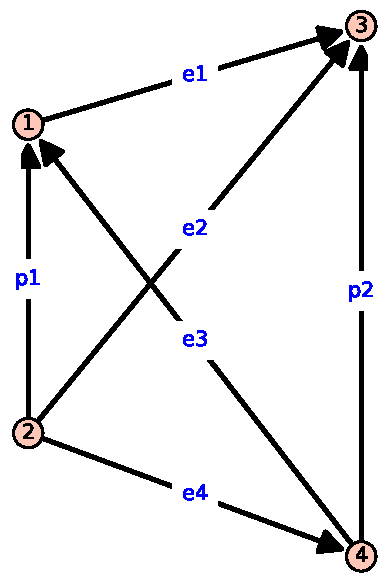
\includegraphics[scale=0.5]{K4.pdf}
\end{figure}

We begin with the familiar incidence matrix representation of K4's matroid.
We delete row 2 and take a representation for the dual that is consistent
with our exterior algebra duality operator (\ref{}):


\[
\left(\begin{array}{cc|cccc}
1 & 0 & -1 & 0 & 1 & 0 \\
-1 & 0 & 0 & -1 & 0 & -1 \\
0 & 1 & 1 & 1 & 0 & 0 \\
0 & -1 & 0 & 0 & -1 & 1
\end{array}\right)
\;\;\;
N_\alpha=
\left(\begin{array}
{cc|cccc}
1 & 0 & -1 & 0 & 1 & 0 \\
0 & 1 & 1 & 1 & 0 & 0 \\
0 & -1 & 0 & 0 & -1 & 1
\end{array}\right)
%\]
\;\;\;\;
%\[
N_\beta^\perp =
\left(\begin{array}{cc|cccc}
1 & 0 & 0 & 0 & -1 & -1 \\
0 & 1 & 0 & -1 & 0 & 1 \\
0 & 0 & 1 & -1 & 1 & 1
\end{array}\right)
\]


We form the following system of equations according to (\ref{LmatrixDef}).

\begin{equation}\label{K4Equation}
\begin{split}
  0=L\left(\begin{array}{cc} {\Nal} \\ {\NbePe}  \end{array}\right)z
    =& \left[\begin{array}{c|c|c} \Nal(P)  &  0  &  \Nal(E)G \\  \hline
        0  & \NbePe(P)  &  \NbePe(E)R \end{array}\right]
    \left[ \begin{array}{c} i_{p_1} \\ i_{p_2} \\ v_{p_1} \\ v_{p_2} \\ x_{e_1} \\ x_{e_2} \\ x_{e_3} \\ x_{e_4}
      \end{array}
      \right]
    \\
    =&
\left(\begin{array}{cc|cc|cccc}
1 & 0 & 0 & 0 & -g_{1} & 0 & g_{3} & 0 \\
0 & 1 & 0 & 0 & g_{1} & g_{2} & 0 & 0 \\
0 & -1 & 0 & 0 & 0 & 0 & -g_{3} & g_{4} \\ \hline
0 & 0 & 1 & 0 & 0 & 0 & -r_{3} & -r_{4} \\
0 & 0 & 0 & 1 & 0 & -r_{2} & 0 & r_{4} \\
0 & 0 & 0 & 0 & r_{1} & -r_{2} & r_{3} & r_{4}
\end{array}\right)z
\end{split}
\end{equation}


The electrical network problem at hand is to determine linear constraints on the
port variables $i_p, v_p$, $p\in P = \{p_1, p_2\}$ imposed by the system.  In other words,
we want a linear map $M$ on the $K$-vector space with basis $P_\alpha, P_\beta$ whose kernel
is the projection of this system's solution space.
Below is a solution.
We set $r_e=1$ for $e\in E$, and $D=g_{1} g_{2} g_{3} + g_{1} g_{2} g_{4} + g_{1} g_{3} g_{4} + g_{2} g_{3} g_{4}$.
\begin{equation}\label{K4Soln}
M\left(\begin{array}{c} i_{p1} \\ i_{p2} \\ v_{p1} \\ v_{p2}
\end{array}\right) =
\left(\begin{array}{cccc}
{\left(g_{1} + g_{2}\right)} {\left(g_{3} + g_{4}\right)} & -g_{2} g_{3} + g_{1} g_{4} & D & 0 \\
-g_{2} g_{3} + g_{1} g_{4} & {\left(g_{1} + g_{3}\right)} {\left(g_{2} + g_{4}\right)} & 0 & D
\end{array}\right)
\left(\begin{array}{c} i_{p1} \\ i_{p2} \\ v_{p1} \\ v_{p2}
\end{array}\right) = 0
\end{equation}


To compute $\ext{L}_E$ from its definition, set 
$z=[\ext{p}_{\alpha 1},\ext{p}_{\alpha 2},\ext{p}_{\beta 1},\ext{p}_{\beta 2},
  \ext{e}_1,  \ext{e}_2,  \ext{e}_3,  \ext{e}_4]^t$
in the right hand side of (\ref{K4Equation}) 
and expand in terms of this basis
the exterior product (in order) of the resulting column's entries.
Finally, we select
the terms that can be expressed as $\ext{T}\ext{e}_1\ext{e}_2\ext{e}_3\ext{e}_4$.  The final
value is the sum of such $\ext{T}$.
Each $\ext{T}$ is the $\wedge$ of unique pair of distinct elements
of $\{\ext{p}_{\alpha 1}, \ext{p}_{\alpha 2}, \ext{p}_{\beta 1}, \ext{p}_{\beta 2}\}$
with a coefficient that is a polynomial in the 
$g_e$, $r_e$.  These coefficients are \Plucker coordinates
for the orthogonal complement of the electrical network
(itself parametrized by the $g_e, r_e$) solution space.
Each polynomial
term encodes a subset of $E=\{e_1, e_2, e_3, e_4\}$, for example, $\{e_1, e_2\}$ is encoded
by $g_1g_2r_3r_4$. Note that each coefficient enumerates
the common bases of a pair of not always distinct of matroid minors.


\begin{equation}\label{K4table}
\begin{array}{|c|c|c|} \hline
\text{basis element} & \text{coefficient} & \text{enumerates bases}\\
  \hline

\ext{p}_{\alpha 1}\ext{p}_{\alpha 2} &
g_1 + g_2 + g_3 + g_4 & \mathcal{B}(G/\{p_1, p_2\})

\\ \hline

\ext{p}_{\alpha 1}\ext{p}_{\beta 1} &
g_2g_3 - g_1g_4 &  \mathcal{B}(G/p_1\setminus p_2)\cap\mathcal{B}(G/p_2\setminus p_1)

\\ \hline

\ext{p}_{\alpha 1}\ext{p}_{\beta 2} &
(g_1 + g_2)(g_3 + g_4) & \mathcal{B}(G/p_1\setminus p_2)
\\ \hline 

\ext{p}_{\alpha 2}\ext{p}_{\beta 1} & -(g_1 + g_3)(g_2+g_4) & \mathcal{B}(G/p_2\setminus p_1)
\\ \hline
 
\ext{p}_{\alpha 2}\ext{p}_{\beta 2} &
-g_2g_3 + g_1g_4 & \mathcal{B}(G/p_1\setminus p_2)\cap\mathcal{B}(G/p_2\setminus p_1)
\\ \hline
 
\ext{p}_{\beta 1}\ext{p}_{\beta 2} &
g_1g_2g_3 + g_1g_2g_4 + g_1g_3g_4 + g_2g_3g_4 & \mathcal{B}(G\setminus \{p_1, p_2\})
\\ \hline

\end{array}
\end{equation}

To verify that the coefficients of our $\ext{L}_E$
in (\ref{K4table}) are \Plucker coordinates, and
indeed that $\ext{L}_E$ represents the space of
linear constraints for the
network solution problem,
one can calculate that each $2\times 2$ minor of the matrix in
(\ref{K4Soln}) equals the $D$ multiple of the corresponding coefficient
in  (\ref{K4table}).  The one non-trivial calculation is
\[
{\left(g_{1} + g_{2}\right)} {\left(g_{1} + g_{3}\right)} {\left(g_{2} + g_{4}\right)} {\left(g_{3} + g_{4}\right)} - {\left(-g_{2} g_{3} + g_{1} g_{4}\right)}^{2} = D(g_1+g_2+g_3+g_4)
\]

This example also demonstrates that $\ext{L}_E$ might not have a
matrix representation all of whose entries are $K_0$ polynomials in the $r_e, g_e$.

\subsection{Example with $\ext{N}_\alpha\neq\ext{N}_\beta$}
We take $N_\alpha$ from before, but form $N_\beta$ from $N_\alpha$ by replacing $-1$s by $0$.
$N_\beta$ now represents the partition matroid $\Pi$ where
each edge in a basis has its head incident to one distinct vertex in $\{1, 3, 4 \}$.


\[
N_\alpha=
\left(\begin{array}
{cc|cccc}
1 & 0 & -1 & 0 & 1 & 0 \\
0 & 1 & 1 & 1 & 0 & 0 \\
0 & -1 & 0 & 0 & -1 & 1
\end{array}\right)
%\]
\;\;\;\;
%\[
N_\beta=
\left(\begin{array}
{cc|cccc}
1 & 0 & 0 & 0 & 1 & 0 \\
0 & 1 & 1 & 1 & 0 & 0 \\
0 & 0 & 0 & 0 & 0 & 1
\end{array}\right)
\;\;\;
N_\beta^\perp =
\left(\begin{array}{cc|cccc}
1 & 0 & 0 & 0 & -1 & 0 \\
0 & 1 & 0 & -1 & 0 & 0 \\
0 & 0 & 1 & -1 & 0 & 0
\end{array}\right)
\]


\begin{equation}\label{K4Dirtable}
\begin{array}{|c|c|c|} \hline
\text{basis element} & \text{coefficient} & \text{enumerates bases}\\
  \hline

\ext{p}_{\alpha 1}\ext{p}_{\alpha 2} &
 g_{4} & \mathcal{B}(G/\{p_1, p_2\}) \cap  \mathcal{B}(\Pi/\{p_1, p_2\})

\\ \hline

\ext{p}_{\alpha 1}\ext{p}_{\beta 1} &
0 &  \mathcal{B}(G/p_1\setminus p_2)\cap\mathcal{B}(\Pi/p_2\setminus p_1)

\\ \hline

\ext{p}_{\alpha 1}\ext{p}_{\beta 2} &
 (g_{1} +  g_{2}) g_{4} & \mathcal{B}(G/p_1\setminus p_2)  \cap \mathcal{B}(\Pi/p_1\setminus p_2)
\\ \hline 

\ext{p}_{\alpha 2}\ext{p}_{\beta 1} &
- g_{3} g_{4} & \mathcal{B}(G/p_2\setminus p_1) \cap \mathcal{B}(\Pi/p_2\setminus p_1)
\\ \hline
 
\ext{p}_{\alpha 2}\ext{p}_{\beta 2} &
 g_{1} g_{4} & \mathcal{B}(G/p_1\setminus p_2)\cap\mathcal{B}(\Pi/p_2\setminus p_1)
\\ \hline
 
\ext{p}_{\beta 1}\ext{p}_{\beta 2} &
 (g_{1} +g_{2}) g_{3} g_{4} & \mathcal{B}(G\setminus \{p_1, p_2\})  \cap \mathcal{B}(\Pi\setminus \{p_1, p_2\})
\\ \hline

\end{array}
\end{equation}









\section{Proof and Corollaries}\label{proofs}

We begin with routine properties used in the proof.

    \begin{prop}
      Let $S$ be the sequenced ground set for $\ext{N}$, $A$ a sequenced subset of
      of the elements of $S$, and $A_\sigma$ be $A$ permuted by $\sigma$.  Let $C, D$ be other sequenced
      sets so $A$, $C$ and $D$ are pairwise disjoint.
      \begin{equation}\label{permuteContraction}
        \ext{N}/A_\sigma = \epsilon(CAD)\epsilon(CA_\sigma D)\ext{N}/A = \text{sign}(\sigma)\ext{N}/A
      \end{equation}
    \end{prop}
    \begin{proof}
      Calculating componentwise from the definition,
      \[
      (\ext{N}/A_\sigma)[B]=\ext{N}[BA_\sigma]=\epsilon(CAD)\epsilon(CA_\sigma D)\ext{N}[BA]=
      \epsilon(CAD)\epsilon(CA_\sigma D)(\ext{N}/A)[B]
      \]
      since $\epsilon(CAD)\epsilon(CA_\sigma D)=\text{sign}(\sigma)$.
    \end{proof}


    \begin{prop}
      For $i=1, 2$, let $S^{i}$ be sequenced ground sets for $\ext{N}^{i}$, pairwise disjoint.
      Let $E^i$ be sequenced sets whose elements satisfy $E^i\subseteq S^i$.
      \begin{equation}\label{distcontractwedge}
        (\ext{N}^1 \wedge \ext{N}^2)/E^1E^2 = (-1)^{(r\ext{N}^2-|E^2|) |E^1|} (\ext{N}^1/E^1 \wedge \ext{N}^2/E^2)
      \end{equation}
    \end{prop}
    \begin{proof}
      Proceeding componentwise, with sequenced $B^i\subseteq S^i\setminus E^i$
      \begin{equation*}
        \begin{split}
      (\ext{N}^1 \wedge \ext{N}^2)/E^1E^2)[B^1B^2]
      &=(\ext{N}^1 \wedge \ext{N}^2))[B^1B^2E^1E^2]
      \\
      &=(-1)^{(|B^2| |E^1|)} (\ext{N}^1 \wedge \ext{N}^2))[B^1E^1B^2E^2]
      \\
      &=(-1)^{(|B^2| |E^1|)} (\ext{N}^1[B^1E^1])( \ext{N}^2[B^2E^2])
      \\
      &=(-1)^{(|B^2| |E^1|)} (\ext{N}^1/E^1[B^1])( \ext{N}^2/E^2[B^2])
      \\
      &=(-1)^{(|B^2| |E^1|)} (\ext{N}^1/E^1 \wedge \ext{N}^2/E^2)[B^1B^2]
        \end{split}
      \end{equation*}
      Since this calculation relevant only for $|B^2|=r\ext{N}^2-|E^2|$, (\ref{distcontractwedge}) follows.
    \end{proof}

\begin{prop}\label{delecontdualprop}
  Let $S$ be the ground set for $\ext{N}$.
  Let $X$ be a sequenced subset of $S$.
  Let $S'$ be any sequencing of $S\backslash X$.
    \begin{equation}\label{dualDelete} (\ext{N}\backslash X)^\perp = \epsilon(S')\epsilon(S'X)(\ext{N}^\perp/X)
    \end{equation}
    \begin{equation}\label{dualContract} (\ext{N}/X)^\perp = \epsilon(S')\epsilon(S'X)(-1)^{|X|r\ext{N}^\perp}(\ext{N}^\perp\backslash X)
    \end{equation}
\end{prop}
\begin{proof}
  Apply the definitions.  These dualization formulas are well-defined since they
  are unchanged over different sequencings of $S'$.
\end{proof}


\newcommand{\Nsup}[1]{\ext{N}^{#1}}
\newcommand{\NsupPerp}[1]{{\ext{N}^{#1}}^\perp}

\begin{prop}
  For $i=1, 2$, let $S^{i}$ be sequenced ground sets for $\ext{N}^{i}$, pairwise disjoint.
  \begin{equation}\label{commutewedgeperp}
    (\Nsup{1}\wedge\Nsup{2})^\perp =
    \epsilon(S^{1})\epsilon(S^{2})\epsilon(S^{1}S^{2})(-1)^{(r{\NsupPerp{1}})( r\Nsup{2})}
        \NsupPerp{1}\wedge\NsupPerp{2}
    \end{equation}
\end{prop}
\begin{proof}
  Calculate componentwise, for any orderings
  $B_i\subseteq S_i$ and $\overline{B_i}\subseteq S_i\setminus B_i$:
  \begin{equation*}
    \begin{split}
      (\Nsup{1}\wedge\Nsup{2})^\perp[B_1B_2]=
      &(\Nsup{1}\wedge\Nsup{2})[\overline{B_1}\;\overline{B_2}]\;
      \epsilon(\overline{B_1}\;\overline{B_2}B_1 B_2)\\
      =&\Nsup{1}[\overline{B_1}]\Nsup{2}[\overline{B_2}]\;\epsilon(\overline{B_1}\;\overline{B_2}B_1 B_2)\\
    =&\{\NsupPerp{1}[B_1]\epsilon(\overline{B_1}B_1)\}\;
    \{\NsupPerp{2}[B_2]\epsilon(\overline{B_2}B_2)\}\;\epsilon(\overline{B_1}\;\overline{B_2}B_1 B_2)\\
    =&(\NsupPerp{1}\wedge\NsupPerp{2})[B_1B_2]\;\epsilon(\overline{B_1}B_1)\epsilon(\overline{B_2}B_2)\epsilon(\overline{B_1}\;\overline{B_2}B_1 B_2)\\
    \end{split}
  \end{equation*}
  Since $|\overline{B_2}|=r\Nsup{2}$ and $|B_1|=r\NsupPerp{1}$,
$%  \[
  \epsilon(\overline{B_1}\;\overline{B_2}B_1 B_2)=(-1)^{r\NsupPerp{1}r\Nsup{2}}\epsilon(\overline{B_1}B_1\;\overline{B_2} B_2)
$. %  \]
  (\ref{commutewedgeperp}) follows since, for $i=1,2$, simutaneously permuting
  the two appearances of $\overline{B_i}B_i$ into $S^{i}$ in the combined sign expresssion does
  not change its sign.
\end{proof}

Remark: The sign $\epsilon(S^{1})\epsilon(S^{2})\epsilon(S^{1}S^{2})$ may seem strange.
The three $\epsilon$'s are functions of sequences from three different sets.  They are
used  in defining $\perp$ of $\Nsup{1}$, $\Nsup{2}$ and $\Nsup{1}\wedge\Nsup{2}$ respectively.
The formula must connect three different positively oriented unit volumes
used to define Hodge star in three different exterior algebras.


\subsection{Tutte Identity Theorems}


\begin{theo}\label{delecontrtheorem}
  Given sequenced $P$ and $E$, for all $e\in E$ and sequenced $E'=E\setminus e$,
  \begin{equation}\label{delecontrequation}
     \epsilon(PE)\extLHorSub{E}{\eNal}{\eNbe}=
      \epsilon(PE')
      \left(
      g_e\extLHorSub{E'}{\eNal/e}{\eNbe/e} +
      r_e\extLHorSub{E'}{\eNal\backslash e}{\eNbe\backslash e}\right)
  \end{equation}
\end{theo}
\begin{proof}
Within each of the two factors in
  \[
   \ext{L} := \ext{L}\left( \begin{array}{c} \eNal\\ \eNbePe \end{array} \right)
=\Is_G(\eNal)\wedge\Vs_R(\eNbePe)
  \]
let us group the terms according to those that don't and those that do
contain $\ext{e}$ as a factor.   Since for the given $e$, 
  $\Vs_R(\ext{e})=r_e\ext{e}$, $\Is_G(\ext{e})=g_e\ext{e}$,
\[
\ext{L} =
\left\{\Is_G(\eNal \backslash e) + (g_e\Is_G(\eNal/e))\ext{e}\right\}
\;\;\bigwedge\;\;
\left\{\Vs_R(\eNbePe\backslash e) + (r_e\Vs_R(\eNbePe/e))\ext{e})\right\}  
\]
Each factor has the form $\{\ext{X} + \ext{Y}\ext{e}\}$ where
$\ext{X}$ (and $\ext{Y}$) are not multiples of $\ext{e}$, so
\[
\ext{L}=
r_e\left\{ (\Is_G(\eNal\backslash e))\wedge (\Vs_R(\eNbePe/e))\ext{e} \right\}  +
g_e\left\{ (\Is_G(\eNal/e))\ext{e})  \wedge (\Vs_R(\eNbePe\backslash e)\right\}
+\ext{J}
\]
where $\ext{J}/E = 0$.
The sign change from commuting $\ext{e}$ with $(\Vs_R(\eNbePe\backslash e)$ gives
\[
\begin{split} 
   \ext{L} = \Big( r_e  \;\;\; \;\;\;\;\;\;\;\;\;\;\;\;\;\; & \Is(\eNal\backslash e)  \wedge (\Vs(\eNbePe/e))      \wedge  \ext{e} \\
   \;\;+ g_e (-1)^{r(\eNbePe)} ( & \Is(\eNal/e))\wedge(\Vs(\eNbePe\backslash e))   \wedge  \ext{e}\Big)
+\ext{J}.\\
\end{split}
\]
With sets $E$ (and $E'=E\setminus e$ used below) given by sequences
which are part of the theorem's data, we contract $E$ to get
%\begin{equation}
\[
\ext{L}_E=\ext{L}/E = r_e\left(\ext{L}\left(\begin{array}{c} \eNal\backslash e \\
    \eNbePe/e  \end{array} \right)  \wedge \ext{e} /E \right) +
   g_e(-1)^{r(\eNbePe)}\left(\ext{L}\left(\begin{array}{c} \eNal /e \\
    \eNbePe \backslash e \end{array} \right) \wedge \ext{e} /E \right).
   \]
On dualizing with (\ref{dualDelete}) and (\ref{dualContract})
   \[
     \ext{N_\beta}^\perp/e  = \epsilon(S')\epsilon(S'e) (\ext{N_\beta}\backslash e)^\perp
     \]
     \[
       \ext{N_\beta}^\perp\backslash e = \epsilon(S')\epsilon(S'e)(-1)^{|\{e\}|r\ext{N\beta}^\perp}(\ext{N_\beta}/e)^\perp,
       \]
we get
\begin{equation}\label{delecontrDEPSprime}
  \ext{L}_E = \epsilon(S')\epsilon(S'e)
  \left[ \ext{L'} \wedge e /E \right],
\end{equation}
where the abbreviation        
\[
\ext{L'} = \left[
        r_e\ext{L}\left(
        \begin{array}{c} \eNal\backslash e \\
    (\eNbe\backslash e)^\perp
    \end{array}  \right) 
+
        g_e\ext{L}\left(
        \begin{array}{c} \eNal / e \\
    (\eNbe / e)^\perp \end{array} \right) 
        \right].
\]




$S'$ is an arbitrary ordering of $P\dunion (E\backslash e)$ introduced
when we dualized $\ext{N_\beta}\backslash e$ and
$\ext{N_\beta}/ e$; the results are independent of this ordering.
We use the same ordering for both dualizations.
Our concluding
step will show that the sign corrections in (\ref{delecontrequation}) depend only
on the orderings of $P$, $E$ and $E'$ from the theorem's data, that is
we must show (\ref{delecontrDEPSprime})
$\ext{L}_E=\epsilon(S')\epsilon(S'e)(\ext{L'}\wedge \ext{e})/E$
implies (\ref{delecontrequation}).

From (\ref{permuteContraction}),
permuting $E$ to $E'e$ changes the sign by $\epsilon(E)\epsilon(E'e)$, so
\[
\ext{L}_E=\epsilon(S')\epsilon(S'e)\epsilon(E)\epsilon(E'e)(\ext{L'}\wedge \ext{e})/(E'e).
\]
Since the ordering $S'$ is arbitrary, take $S'=PE'$, to get
\[
\ext{L}_E=\epsilon(PE')\epsilon(PE'e)\epsilon(E)\epsilon(E'e)(\ext{L'}\wedge \ext{e})/(E'e).
\]
We now simulaneously permute the two appearances of $E'e$ to $E$ and verify ((\ref{delecontrequation}):
\[
\ext{L}_E=\epsilon(PE')\epsilon(PE)\epsilon(E)\epsilon(E)(\ext{L'}\wedge \ext{e})/(E'e)
=\epsilon(PE')\epsilon(PE)(\ext{L'}\wedge \ext{e})/(E'e).
\]
\end{proof}




\begin{theo}\label{producttheorem}
Given, for $i = 1, 2$,
  $\ext{N}_\alpha^{i}$,  $\ext{N}_\beta^{i}$, ${\ext{N}_\beta^{i}}^\perp$ 
  and
  sequenced $E=E^{1}\dunion E^{2}$, $P^{i}$, $E^{i}$,
  \begin{equation}\label{productequation}
    \begin{split}
    \epsilon(P^1P^2E)
    &\LHorSub{E}
            {(\ext{N}_\alpha^{1}\wedge\ext{N}_\alpha^{2})}
            {(\ext{N}_\beta^{1}\wedge\ext{N}_\beta^{2})}
    = \\
    \epsilon(P^{1}E^{1})
    \epsilon(P^{2}E^{2}) 
        &\left(\LHorSub{E^{1}}{\ext{N}_\alpha^{1}}{\ext{N}_\beta^{1}}
        \wedge
        \LHorSub{E^{2}}{\ext{N}_\alpha^{2}}{\ext{N}_\beta^{2}}
          \right)
    \end{split}
  \end{equation}
\end{theo}

\begin{proof}

Using (\ref{commutewedgeperp}),
\begin{equation*}
  \begin{split}
    \ext{L} := & \ext{L}\left(
    \begin{array}{c}
      \ext{N}^{1}_\alpha\wedge \ext{N}^{2}_\alpha
      \\     
      (\ext{N}^{1}_\beta\wedge\ext{N}^{2}_\beta)^\perp
    \end{array} \right)
  =\Is_G(\ext{N}_\alpha^{1}\wedge \ext{N}_\alpha^{2})
  \wedge\left(\Vs_R({\ext{N}_\beta}^{1}\wedge{\ext{N}_\beta}^{2})\right)^\perp
  \\
  =&
  \Is_G(\ext{N}_\alpha^{1})\wedge \Is_G(\ext{N}_\alpha^{2})
  \wedge\Vs_R({\ext{N}_\beta^{1}}^\perp)\wedge\Vs_R({\ext{N}_\beta^{2}}^\perp)
  \epsilon(S^{1})\epsilon(S^{2})\epsilon(S^{1}S^{2})(-1)^{(r{\ext{N}_\beta^{1}}^\perp)( r{\ext{N}_\beta}^{2})}
  \\
  =& 
    \Is_G(\ext{N}_\alpha^{1}) \wedge \Vs_R({\ext{N}_\beta^{1}}^\perp) \wedge
    \Is_G(\ext{N}_\alpha^{2}) \wedge \Vs_R({\ext{N}_\beta^{2}}^\perp)
    \epsilon(S^{1})\epsilon(S^{2})\epsilon(S^{1}S^{2})
  \end{split}
\end{equation*}
since $(-1)^{(r{\ext{N}_\beta^{1}}^\perp)( r{\ext{N}_\beta}^{2})} \ext{N}_\alpha^{2} {\ext{N}_\beta^{1}}^\perp
={\ext{N}_\beta^{1}}^\perp \ext{N}_\alpha^{2}$.  By (\ref{permuteContraction})
$
\ext{L}/E = \epsilon(E)\epsilon(E^{1} E^{2})\ext{L}/E^{1}E^{2},
$ so
\[
\ext{L}/E = \epsilon(E)\epsilon(E^{1} E^{2})\epsilon(S^{1})\epsilon(S^{2})\epsilon(S^{1}S^{2})
\left(
 \Is_G(\ext{N}_\alpha^{1}) \wedge \Vs_R({\ext{N}_\beta^{1}}^\perp) \wedge
    \Is_G(\ext{N}_\alpha^{2}) \wedge \Vs_R({\ext{N}_\beta^{2}}^\perp)
\right)/E^1E^2
\]
\[
=\epsilon(E)\epsilon(E^{1} E^{2})\epsilon(S^{1})\epsilon(S^{2})\epsilon(S^{1}S^{2})
(-1)^{(r\ext{N}^2-|E^2|)(|E^1|)}
\left(\LHorSub{E^{1}}{\ext{N}_\alpha^{1}}{\ext{N}_\beta^{1}}
        \wedge
        \LHorSub{E^{2}}{\ext{N}_\alpha^{2}}{\ext{N}_\beta^{2}}
          \right)
          \]
by (\ref{distcontractwedge}) so we are done except to verify the sign correction.  With $S^i=P^iE^i$ the sign is
\[
\epsilon(E)\epsilon(E^{1} E^{2})\epsilon(P^1E^1)\epsilon(P^{2}E^2)\epsilon(P^1E^1P^2E^2)
(-1)^{(r\ext{N}^2-|E^2|)(|E^1|)}
\]
\[
=\epsilon(E)\epsilon(E^{1} E^{2})\epsilon(P^1E^1)\epsilon(P^{2}E^2)\epsilon(P^1P^2E^1E^2).
\]
We now obtain correction of (\ref{productequation}) by simultaneously permuting the two occurrances of $E^1E^2$
to $E$:
\[
\epsilon(E)^2\epsilon(P^1E^1)\epsilon(P^{2}E^2)\epsilon(P^1P^2E)
\]



\end{proof}

This corollary is very helpful for calculations.

\begin{coro}
  Suppose all elements that could be included in sets we denote by $P$ or $E$ are linearly ordered,
  elements that can be in $P$ are each before elements that can be in $E$,
  and each subset of such elements is considered to be sequenced in increasing order.  With
  $E$, $P$, $\ext{N_\alpha}$, $\ext{N_\beta}$ and $e\in E\setminus P$ as above
  \begin{equation}
       \extLHorSub{E}{\eNal}{\eNbe}=
      g_e\extLHorSub{E\setminus e}{\eNal/e}{\eNbe/e} +
      r_e\extLHorSub{E\setminus e}{\eNal\backslash e}{\eNbe\backslash e}
  \end{equation}
\end{coro}
\begin{proof}
  Use for $\epsilon$ the orientation for which every increasing sequence is positive.
\end{proof}

\section{Towards a Tutte Polynomial}\label{polys}

\newcommand{\V}{v}
\newcommand{\W}{w}


An easy consequence of Theorem \ref{delecontrtheorem} is that $\ext{L}_E(\ext{N}_\alpha;\ext{N}_\beta)$ has an
expansion over the common bases of the matroids represented by $\ext{N}_\alpha$ and $\ext{N}_\beta$.

\begin{defi}\label{NcontrArestrictP}
For $A\subseteq E$, the abbreviation $\ext{N}/A|P$ $=$
$\ext{N}/A\backslash \overline{A}$, \\
where $\overline{A}=(S(\ext{N})\setminus P)\setminus A$.  The analgous
abbreviation for matroids is \\
$\mathcal{N}/A|P$ $=$
$\mathcal{N}/A\backslash \overline{A}$.
\end{defi}

Notice that in the expansion below, the only non-zero terms in the sums are those for which $A$ is a common
basis in the matroids represented by $\ext{N}_\alpha/Q_\alpha$ and $\ext{N}_\beta/Q_\beta$.
Because of our definition of contraction,
if $Q_\alpha, Q_\beta$ are not independent sets in the matroids of $\ext{N}_\alpha, \ext{N}_\beta$
respectively, the term will be zero.


\begin{coro}\label{commonbasescoro}
  Given 
  equal length sequences $Q_\alpha \subseteq P$, $Q_\beta \subseteq P$,
  let $\overline{Q_\beta}=P\setminus Q_\beta$.
\label{common-basis-expansion}
\begin{equation}
  \begin{split}
    \epsilon(  Q_\beta \overline{Q_\beta} )\epsilon(PE)
    \extLHorSub{E}{\eNal}{\eNbe}  [Q_{\alpha}\overline{Q_{\beta}}]
    =& 
    \epsilon(P)\sum_{A\subseteq E}
    (\ext{N}_\alpha/A|P) [Q_\alpha]
    (\ext{N}_\beta/A|P) [Q_\beta] g_Ar_{\overline{A}} \\
    =& 
    \epsilon(P)\sum_{A\subseteq E}
    \ext{N}_\alpha[Q_\alpha A]
    \ext{N}_\beta [Q_\beta A]
    g_Ar_{\overline{A}}.
%    \\
%    \epsilon(  Q_\alpha \overline{Q_\beta} )\epsilon(PE)
%    \extLHorSub{E}{\eNal}{\eNbe}  
%    =&
%       \epsilon(P)\sum_{A\subseteq E}
%    (\ext{N}_\alpha/A|P)\wedge
%    (\ext{N}_\beta/A|P)
%    g_Ar_{\overline{A}}
  \end{split}
\end{equation}

\end{coro}


\begin{proof}
  By induction on (\ref{productequation}),
  \[
  \extLHorSub{E}{\eNal}{\eNbe}  [Q_{\alpha}\overline{Q_{\beta}}] = \epsilon(P)\epsilon(PE)
  \sum_{A\subseteq E}\extLHorSub{\emptyset}{\ext{N}_\alpha/A|P}{\ext{N}_\beta/A|P}[Q_{\alpha}\overline{Q_{\beta}}]
  g_Ar_{\overline{A}}.
  \]
By definitions \ref{LDefs} and \ref{iGvRdefs}, 
  \[
\extLHorSub{\emptyset}{\ext{N}_\alpha/A|P}{\ext{N}_\beta/A|P}[Q_{\alpha}\overline{Q_{\beta}}]
=(\ext{N}_\alpha/A|P)[Q_\alpha](\ext{N}_\beta/A|P)^\perp[\overline{Q_{\beta}}].
\]
Dualization
$(\ext{N}_\beta/A|P)^\perp[\overline{Q_{\beta}}]=
(\ext{N}_\beta/A|P)[Q_{\beta}]\epsilon(Q_{\beta}\overline{Q_{\beta}})$
gives the first equation.
Our definition of contraction gives the second.
\end{proof}





Here we show:  $\ext{L}_E$ is an evaluation of a common generalization
of parametrized Tutte polynomials, relative Tutte polynomials and linking
(matroid pair Tutte) polynomials.
Based on these origins, it is straightforward to demonstrate the Tutte
identities this generalization satisfies (Theorem \ref{pairbigtuttepolytheorem}.)
This Tutte polynomial has matroid
variables, and the ones that appear in the polynomial for a given
pair of matroids are minors of those matroids.
However, when the
matroid minors in the generalization are replaced by exterior algebra minors, the Tutte
equations fail to be satisfied.  The only situation where
those Tutte equations are satisfied is when the corank and nullity
variables are set to zero and the matroids are unimodular (i.e. regular).

Let $\mathcal{N}$ be a matroid.  In the following, $\MVar{\mathcal{N}}$ will
denote the product of the connected components of $\mathcal{N}$, each regarded as
a variable.

We will use the term ``$P$-ported'' for what has been called ``set-pointed'' and
``relative'' Tutte functions and polynomial. The following combines known definitions:
\begin{enumerate}
\item
  Las Vergnas' ``big'' Tutte polynomial of a $P$-ported matroid.  Our
references\cite{MR0419272,SetPointedLV,sdcPorted,TutteEx,RelTuttePolyDiaoHetyei}
document that all the fundamental features
(expansions, universality, etc.)
of Tutte function theory extend to porting/set-pointing/relativization.
\item
  ``Normal'' parametrized Tutte functions which
  are those that have rank-nullity generating function interpretations,
  according
to classifications given by Zaslavsky\cite{MR93a:05047},
and Bollobas and Riordan\cite{BollobasRiordanTuttePolyColored}, and
unified by Monaghan and Traldi\cite{Ellis-Monaghan-Traldi}.
\item Welsh and Kayibi's linking polynomial of a matroid pair\cite{WelshKayibiLinking}.
\end{enumerate}
  
\begin{defi}
\begin{equation}\label{bigportedpairpolydef}
  \begin{split}
    L_E(\mathcal{N}_\alpha,\mathcal{N_\beta};\text{... matroid variables } &
    , \text{...};
    \V_\alpha,\W_\alpha,\V_\beta,\W_\beta) \\
    =\sum_{A\subseteq E}\MVar{\mathcal{N}_\alpha/A|P}\MVar{\mathcal{N}_\beta/A|P}
& g_A r_{\overline{A}} \\
& \V_\alpha^{r_\alpha(\mathcal{N}_\alpha)-r_\alpha(\mathcal{N}_\alpha/A|P)-r_\alpha(A)} 
 \W_\alpha^{|A|-r_\alpha(A)} \\
& \V_\beta^{r_\beta(\mathcal{N}_\beta)-r_\beta(\mathcal{N}_\beta/A|P)-r_\beta(A)} 
 \W_\beta^{|A|-r_\beta(A)}  \\
 =
 \sum_{A\subseteq E}\MVar{\mathcal{N}_\alpha/A|P}\MVar{\mathcal{N}_\beta/A|P}
 & g_A r_{\overline{A}} \\
 & \V_\alpha^{r_\alpha(\mathcal{N}_\alpha)-r_\alpha(P\cup A)} 
 \W_\alpha^{|A|-r_\alpha(A)} \\
& \V_\beta^{r_\beta(\mathcal{N}_\beta)-r_\beta(P \cup A)} 
 \W_\beta^{|A|-r_\beta(A)}. 
  \end{split}
\end{equation}
\end{defi}

Welsh and Kayibi's linking polynomial is obtained by taking $P=\emptyset$ and
all $r_e=g_e=1$ in the above.  (Also, they use $x-1 = \V_\alpha$, $y-1 = \W_\alpha$,
$u-1=\V_\beta$ and $v-1=\W_\beta$.)


The feature of normal Tutte polynomials manifest in this definition
is that
our variables $\V_\alpha$,
$\V_\beta$, $\W_\alpha$, and $\W_\beta$ are independent of $e$.
The cited references prove that the coloop and loop values
for $e\not\in P$ must be evaluations of
our definitions' expressions with these four
variables  in order
for the polynomial to be a Tutte function (i.e., satisfy the
parametrized Tutte equations over a class of matroids and parameters)
\emph{and}
have a corank-nullity expansion.


\begin{theo}\label{pairbigtuttepolytheorem}
  \begin{equation*}
    \begin{array}{cc|rl}
      
      e \text{ in }N_\alpha  & e \text{ in }N_\beta &
      \multicolumn{2}{c}{L_E(\mathcal{N}_\alpha,\mathcal{N}_\beta)=} \\ \hline \hline
      

          
      \text{non-separator} & \text{non-separator} &
      g_e L_{E'}(\mathcal{N}_\alpha/e,  \mathcal{N}_\beta/e) &+
      r_e L_{E'}(\mathcal{N}_\alpha\backslash e,  \mathcal{N}_\beta \backslash e) \\ \hline
      



      \text{non-separator} & \text{coloop} &
      g_e L_{E'}(\mathcal{N}_\alpha/e,  \mathcal{N}_\beta/ e) &+
      r_e \V_\beta L_{E'}(\mathcal{N}_\alpha\backslash e,  \mathcal{N}_\beta \backslash^\dag e) \\  \hline
      
      \text{non-separator} & \text{loop} &
           g_e \W_\beta L_{E'}(\mathcal{N}_\alpha/e,  \mathcal{N}_\beta/^\dag e) &+
           r_e L_{E'}(\mathcal{N}_\alpha\backslash e,  \mathcal{N}_\beta \backslash e) \\  \hline
           
      \text{coloop} & \text{non-separator} &
      g_e L_{E'}(\mathcal{N}_\alpha/ e,  \mathcal{N}_\beta/e) &+
      r_e \V_\alpha L_{E'}(\mathcal{N}_\alpha\backslash^\dag e,  \mathcal{N}_\beta \backslash e) \\  \hline
      

      \text{loop} & \text{non-separator} &
           g_e \W_\alpha L_{E'}(\mathcal{N}_\alpha/^\dag e,  \mathcal{N}_\beta/e) &+
           r_e L_{E'}(\mathcal{N}_\alpha\backslash e,  \mathcal{N}_\beta \backslash e) \\  \hline
           




      \text{coloop} & \text{coloop} &
      g_e L_{E'}(\mathcal{N}_\alpha/ e,  \mathcal{N}_\beta/ e) &+
      r_e \V_\alpha \V_\beta L_{E'}(\mathcal{N}_\alpha\backslash^\dag e,  \mathcal{N}_\beta \backslash^\dag e) \\
      & &
      \multicolumn{2}{c}{=( r_e \V_\alpha \V_\beta + g_e) L_{E'}(\mathcal{N}_\alpha- e,  \mathcal{N}_\beta - e)} \\  \hline
      
      \text{coloop} & \text{loop} &
           g_e \W_\beta L_{E'}(\mathcal{N}_\alpha/e,  \mathcal{N}_\beta/^\dag e) &+
           r_e \V_\alpha L_{E'}(\mathcal{N}_\alpha\backslash^\dag e,  \mathcal{N}_\beta \backslash e) \\
           & &
           \multicolumn{2}{c}{=( r_e \V_\alpha + g_e \W_\beta) L_{E'}(\mathcal{N}_\alpha- e,  \mathcal{N}_\beta - e)} \\  \hline
           
      \text{loop} & \text{coloop} &
     g_e \W_\alpha L_{E'}(\mathcal{N}_\alpha/^\dag e,  \mathcal{N}_\beta/e) &+
     r_e \V_\beta L_{E'}(\mathcal{N}_\alpha\backslash e,  \mathcal{N}_\beta \backslash^\dag e) \\
     & &
     \multicolumn{2}{c}{=(r_e \V_\beta + g_e \W_\alpha) L_{E'}(\mathcal{N}_\alpha- e,  \mathcal{N}_\beta - e)} \\  \hline
     
      \text{loop} & \text{loop} &
           g_e \W_\alpha \W_\beta L_{E'}(\mathcal{N}_\alpha/^\dag e,  \mathcal{N}_\beta/^\dag e) &+
           r_e L_{E'}(\mathcal{N}_\alpha\backslash e,  \mathcal{N}_\beta \backslash e) \\   
           & &
           \multicolumn{2}{c}{= (r_e + g_e \W_\alpha \W_\beta) L_{E'}(\mathcal{N}_\alpha - e,  \mathcal{N}_\beta - e)} \\  \hline
 

    \end{array}
  \end{equation*}

  For $e\in E$,
  $\mathcal{N}\backslash^\dag e$ and $\mathcal{N}/^\dag e$ denote that
  $e$ is a separator in $\mathcal{N}$.  In that case,
  $\mathcal{N}\backslash e$ $=$ $\mathcal{N}/ e$ is also
  denoted by $\mathcal{N}- e$.  Furthermore,
  $\mathcal{N}/(A\backslash e)|P$ $=$ $\mathcal{N}/(A \cup e)|P$ $=$ 
  $\mathcal{N}/A|P$.

\end{theo}

\begin{proof}
  Apply straightforward adaptions of proofs given by the aforementioned
  authors, which use the following elementary properties of separators $e$.
  Let $e \not\in A$.  When $e$ is a coloop,
  \[
  r(\mathcal{N})-r_{\mathcal{N}}(A\cup e \cup P)
  =  r(\mathcal{N}-e)-r_{\mathcal{N}-e}(A \cup P)
  \]
  \[ r(\mathcal{N})-r_{\mathcal{N}}(A \cup P)
  =  1+r(\mathcal{N}-e)-r_{\mathcal{N}-e}(A \cup P)
  \]
  \[
  |A\cup e|-r_{\mathcal{N}}(A \cup e \cup P)
   =
   |A|-r_{\mathcal{N}}(A \cup P)
     =
     |A| - r_{\mathcal{N}-e}(A \cup P).
  \]
When $e$ is a loop,
  \[
  r(\mathcal{N})-r_{\mathcal{N}}(A\cup e \cup P)
  =  r(\mathcal{N})-r_{\mathcal{N}}(A \cup P)
  =   r(\mathcal{N}-e)-r_{\mathcal{N}-e}(A \cup P)
  \]
  and
  \[
  |A\cup e|-r_{\mathcal{N}}(A \cup e \cup P)
   =
   1+ |A|-r_{\mathcal{N}-e}(A \cup P)
   \]
   \[
    |A|-r_{\mathcal{N}}(A \cup P)
     =
     |A| - r_{\mathcal{N}-e}(A \cup P).
    \]
\end{proof}
  

\subsection{Counterexample}


It is tempting to investigate whether the expansion identities
of Theorem \ref{pairbigtuttepolytheorem} are satisfied, when the matroid
minor operations are replaced by our exterior algebra minor operations,
by some function of exterior algebra pairs $(\ext{N}_\alpha, \ext{N}_\beta)$.
After all, Theorem \ref{delecontrtheorem} tells us the identities are
satisfied for $\ext{L}_E(\ext{N}_\alpha;\ext{N}_\beta)$ when we set
$v_\alpha=v_\beta=w_\alpha=w_\beta=0$.  The simplest example, where $P=\emptyset$,
reveals the answer is no.

Let $\ext{N}_\alpha = a \ext{e}_1 + b \ext{e}_2$ and
$\ext{N}_\beta = c \ext{e}_1 + d \ext{e}_2$.  Expansion in the
order of $e_1, e_2$ gives the result
\[
g_1 g_2 w_\alpha w_\beta a c + g_1r_2 a c + r_1 g_2 b d + r_1 r_2 v_\alpha v_\beta b d
\]
but in the order $e_2, e_1$ the result is
\[
g_1 g_2 w_\alpha w_\beta b d + g_1r_2 a c + r_1 g_2 b d + r_1 r_2 v_\alpha v_\beta a c
\]

As expected, the results are equal when the $w$'s and $v$'s are set to zero.
Equality holds iff $ac=bd$, so it fails when
$\ext{N}\alpha = \ext{e_1} + \ext{e}_2$ and
$\ext{N}\alpha = \ext{e_1} - \ext{e}_2$, which are unimodular matroid representations.
It also fails for
$\ext{N}_\alpha = \ext{N}_\beta = \ext{e}_1 + 2\ext{e}_2$.



\subsection{When $\ext{L}_E$ is a Tutte polynomial evaluation}
When the exterior algebra elements $\ext{N}_\alpha$ and $\ext{N}_\beta$ are
unimodular representations of (oriented) matroids matroids,  we can take the
matroid variables to encode oriented matroid representations by chirotopes $\chi$
in which one of chirotopes $\pm \chi$ is distinguished.  Then, we can identify
these oriented matroid representations with the above  $\ext{N}_\alpha$ and $\ext{N}_\beta$.
In this situation, $\ext{L}_E(\ext{N}_\alpha;\ext{N}_\beta)$ is the result
of substituting $\ext{N}_\alpha/A|P$ and $\ext{N}_\beta/A|P$ for the matroid
variables in \ref{bigportedpairpolydef}, together with setting the $v$'s and $w$'s to zero.

\section{Discussion and Summary}\label{discussion}


Among the many currently active research subjects
are algebraic theories for variations of
Tutte decomposition and functions, and convolutions for
Tutte functions of various compositions of objects.  
For example,
Krajewski, Moffatt and Tanasa give a common Hopf algebra framework
for the deletion and contraction operations for many of
these variations\cite{MoffatHopfTutte}.
This approach was generalized and further systemized by
Dupont, Fink and Moci\cite{ALCO_2018__1_5_603_0}.
See also Crapo and Schmitt's work
on the Hopf algebra of matroids and call
for attention to ``naturally occurring algebraic
structures'' in matroid theory\cite{CRAPO20051066}.  

Our motivating linear algebra construction, applied to
electrical netwoks, and its the matroid
abstraction
doesn't appear to be addressed in the above cited literature.
Current research along these lines is in Laplacians and their
determinants of simplicial complexes of dimensions greater than 1.

We see our contribution is to Tutte functions of objects like these
when they have ports.  


One of the
first applications of combinatorial enumeration
appeared in a little known 1847 paper by Kirchhoff\cite{Kirchhoff}
in which a solution was given in terms of tree enumerations,
and proven by a graphic matroid basis exchange argument, rather
than by the matrix tree theorem.
Our linear algebra construction and its application to
electrical networks was studied early on by
Bott and Duffin's\cite{BottDuffinAlgNetworks} study of the ``constrained
inverse''.  When the $g_e$, $r_e$ parameters are algebraically independent,
$\LVert{\eNal}{\eNbePe}$\ref{LDefs} represents a minor of a matroid union--
a discusson that relates this to the constrained
inverse appears in \cite{sdcBDIMatroid}.  A product formula for
the $P$-ported Tutte polynomial of a matroid union appears in
\cite{sdcPorted}.  

---------------------------------------
\newpage

The target for us
is exterior algebras, which occur naturally when problems of
partial solution of systems of linear equations\cite{ExteriorAlgInLinalgRef},
i.e., Schur complements,
%of linearly parametrized systems,
are studied from a matroid theory, sometimes oriented, point of view.
In exterior algebra, unlike commutative algebras,
linear subspaces (as matroid representations and
solutions to systems of homogeneous linear equations)
are represented by exterior products of vectors; also called
\emph{decomposible} elements, \emph{decomposibles},
or ``pure'' antisymmetric tensors $\ext{N}$.
When $\ext{N}$ is expanded in terms of the basis
generated by the elements corresponding to a matroid
ground set, the result is a basis enumeration.


Our motivating example of such subspaces occur
in problems posed from graphs that generalize inversion
of graph Laplacians.  These are defined in
terms of linear resistive linear electrical networks,
under Kirchhoffs' and Ohm's laws.





An examination shows that our notion of  $\ext{N}$ and definitions $\ext{N}^\perp$ and $\ext{L}_E$ make
sense even when $\ext{N}$ is a arbitrary element of the exterior algebra, not necessarilly a pure element.
Furthermore, the properties and Tutte identity theorems hold in this wider context.   Of course,
non-pure elements do not represent subspaces, so our matroid representation and subspace
interpretions no longer apply.  On the other hand, a chirotope of any oriented matroid can be encoded by
the sum over the bases of an ordered product of the basis elements.



-------------------------------------



\newpage

-----------------------------------

The oriented matroid abstraction of objects like $\ext{N}$ and values of $\ext{L}_E$
(when $K_0$ is ordered) is an oriented matroid with one of its two chirotopes $\pm \chi$ distinguished; that
distinguished chirotope is $\chi(B) = \text{sign}(\ext{N}[B])$.

Consider definition (\ref{LDefs}) and Theorems (\ref{delecontrtheorem},\ref{producttheorem})
restricted to totally unimodular representations of unimodular (i.e., regular) oriented matroids
with a distinguished chirotope.  In this situation,  $\chi(B) = \ext{N}[B]\in \{0,\pm 1\}$.
So restricted, these definitions and theorems constitute a special case
of a common generalization of three Tutte polynomial variations:
set-pointed/relative/ported Tutte polynomial
Tutte polynomials, 
Bollobos and Riordan's parameterized or colored Tutte polynomials\cite{BollobasRiordanTuttePolyColored},
and Welsh and Kayibi's linking
polynomial of a matroid pair\cite{WelshKayibiLinking}. The idea of set-pointed Tutte polynomials
was likely first recoginzed by Las Vergnas\cite{MR0419272}
and was subsequently rediscovered and developed\cite{sdcPorted,SetPointedLV,RelTuttePolyDiaoHetyei}.
The common feature is an enumeration
of the common bases in a pair of oriented matroids.  Definition (\ref{LDefs}) is a function between
exterior algebras, but the three variations give polynomial functions of matroids.  In our special
case, (\ref{LDefs}) is a evaluation of this common generalization polynomial. 


For general $\ext{N}$ and the matroids they represent, given two indepentent sets $A$ and $A'$,
$\ext{N}/A|P$ and $\ext{N}/A'|P$ might represent the same matroid but may be
different decomposibles and even represent different elements of Grassmannians of $K^{P}$.
Then there is no map from matroids to decomposibles whose evaluation on the ported
Tutte polynomial gives the value of $\ext{L}_E( \ext{N} ; \ext{N} )$.  The basis
expansion of $\ext{L}_E$ for general $\ext{N_\alpha}$, $\ext{N_\beta}$ we do have is
essentially the Cauchy-Binet theorem:


Las Vergnas defined the big Tutte polynomial\cite{} of a set-pointed matroid
as follows, in our notation\cite{} where we called the matroid ``ported''
because of our application to electrical networks.  Each connected matroid
is considered to be a variable and the symbol $\MVar{\mathcal{N}}$ denotes
the product of the connected components of matroid $\mathcal{N}$.

\begin{equation}
  r_{P}(\mathcal{N}) = \sum_{A\subseteq E}\MVar{\mathcal{N}/A|P}
  V^{r(\mathcal{N}) - r(\mathcal{N}/A|P) -r(X)}
  W^{|A|-r(A)}
\end{equation}



Welsh and Kayibi\cite{WelshKayibiLinking} defined (our notation):
\begin{defi}
  Let $\mathcal{N}_\alpha, \mathcal{N}_\beta$ be matroids on $S$ with rank
  functions $r_\alpha$ and $r_\beta$ respectively.  Define the 4-variable
  polynomial $Q$ by
  \begin{equation}
\begin{split}
    Q(\mathcal{N}_\alpha, \mathcal{N}_\beta;x, y, u, v) =
  \sum_{A\subseteq S}
  &(x-1)^{r_\alpha(S)-r_\alpha(A)}
  (y-1)^{|A|-r_\alpha(A)}       \\
  &(u-1)^{r_\beta(S)-r_\beta(A)}
  (v-1)^{|A|-r_\beta(A)}
\end{split}
  \end{equation}
\end{defi}


Let us combine these constructions and obtain the polynomial below whose
variables include the parameters $g_e, r_e$ for $e\in E$:



-----------------








Tutte functions are a well-known, long-standing contstruction
for which new applications, variations and generalizations
continue to be active research subjects. For example,
Krajewski, Moffatt and Tanasa give a common Hopf algebra framework
for the deletion and contraction operations for many of
these variations\cite{KRAJEWSKI2018271}.
This approach was generalized and further systemized by
Dupont, Fink and Moci\cite{UnivTutteCharCombCoalgDupontFinkMoci}.
See also Crapo and Schmitt's work
on the Hopf algebra of matroids and call
for attention to ``naturally occurring algebraic
structures'' in matroid theory\cite{CRAPO20051066}.  The target for us
is exterior algebras, which occur naturally when problems of
partial solution of systems of linear equations\cite{ExteriorAlgInLinalgRef},
i.e., Schur complements,
%of linearly parametrized systems,
are studied from a matroid theory, sometimes oriented, point of view.
In exterior algebra, unlike commutative algebras,
linear subspaces (as matroid representations and
solutions to systems of homogeneous linear equations)
are represented by exterior products of vectors; also called
\emph{decomposible} elements, \emph{decomposibles},
or ``pure'' antisymmetric tensors $\ext{N}$.
When $\ext{N}$ is expanded in terms of the basis
generated by the elements corresponding to a matroid
ground set, the result is a basis enumeration.
Our motivating example of such subspaces occur
in problems posed from graphs that generalize inversion
of graph Laplacians.  These are defined in
terms of linear resistive linear electrical networks,
under Kirchhoffs' and Ohm's laws.  One of the
first applications of combinatorial enumeration
appeared in a little known 1847 paper by Kirchhoff\cite{Kirchhoff}
in which a solution was given in terms of tree enumerations,
and proven by a graphic matroid basis exchange argument, rather
than by the matrix tree theorem.

To connect this with Tutte decomposition, we make
minor notational variations to the machinery of exterior algebra,
also called Grassmann algebra,
as presented by Marcus\cite{MarcusFDMuAlPt2}.  First, we specify the particular basis $S$
so that a decomposible in the exterior algebra generated by $S$
can represent a matroid with ground set $S$.
Second, since we study the solution space projected
into a subspace of distinguished coordinates, we
specify a distinguished subset $P\subseteq S$
and our Tutte function will be valued in exterior algebras generated by sets related to $P$.
Third, as we will see, since dualization by Hodge star is needed,
an orientation must be specified for each space.
Our identities are on pseudo-forms or pseudo-vectors\cite{Frankel}.
So corrections depending on by those orientations
are required in our Tutte identities.  In all, the above projection plus
parametrization of
electrical networks by resistance $r_e$ and/or conductance $g_e$ values
leads us to parametrized Tutte functions with a
restricted Tutte decomposition identity:
\begin{equation}\label{ParamTutteEqGeneric}
   F(N) = g_eF(N/e)+r_eF(N\backslash e) \text{ if\ }e\text{ can be deleted and contracted, and }e\not\in P.
\end{equation}

Our results for single $\ext{N}$ were originally announced in 2006\cite{TutteEx}, but
their extension to
pairs is new.  Beside from their being an exterior algebra 
special case of Welsh and Kayibi's Tutte-like ``linking'' polynomial of
a pair of matroids\cite{WelshKayibiLinking},
we summarize the electrical engineering circuit theory motivation.
When taking an arbitrarilly oriented labelled multigraph for
a matroid theory style model of an electrical network, one
uses coordinates
for voltage drops across edges and current flows through
edges.  Kirchhoff's laws postulate that such currents and voltages
belong to (KCL) the graph's cycle space and (KVL) its orthogonal complement, respectively.
However, in circuit theory applicable to electronics\cite{OzawaPrinPartn},
some graph models are used
of which the linear spaces for voltages and currents are not orthogonal.
For example, to model an ideal (so-called operational) amplifier, one
can postulate that in a graph to which Kirchhoff's laws apply,
both the current and voltage of the amplifier's input edge are zero
and both those quantities of the output edge are not constrained.  Such
models are equivalent to using two graphs (the same when there are no amplifiers)
with common edge labels:  The ``voltage graph''
and the ``current graph''.\footnote{
These two graphs are minors of a common graph, so the pair can be considered
to be a matroid perspective as studied by Las Vergnas\cite{SetPointedLV}.}
The equations are comprised of KCL from the current graph, KVL from
the voltage graph and Ohm's law to relate current to voltage in
each resistor.  We have related oriented matroid properties of
such graph pairs to questions of well-posedness of electrical
circuit theory problems\cite{sdcOMP}.  This is the origin of our investigations of
(\ref{ParamTutteEqGeneric})  where the object $\ext{N}$ is generalized
to a \emph{pair} $\ext{N}_\alpha$, $\ext{N}_\beta$, corresponding to the ``current graph''
and ``voltage graph'' respectively.  One result is that the solution problem
is well-posed for generic resistance parameters iff the two graphs have a common
spanning tree.  A much more familiar instance is the matrix tree theorem
for directed graphs. Its proof by the Cauchy-Binet theorem reveals that
the enumerated rooted arborescences are the common bases in the graphic
matroid and the partition matroid on edges that encodes the edge head and vertex
incidences.  Thus (\ref{ParamTutteEqGeneric}) becomes
\begin{equation}\label{ParamTutteEqGenericPairs}
  F(\ext{N}_\alpha\;\;\ext{N}_\beta) =
  g_eF(\ext{N}_{\alpha}/e\;\;\ext{N}{_\beta}/e)+
  r_eF(\ext{N}_{\alpha}\backslash e\;\;\ext{N}_{\beta}\backslash e) 
\end{equation}
if $e$ can be deleted and contracted, and $e\not\in P$.





One of the earliest Tutte functions is the basis enumerator for matroids. It
is a determinant in the case of graphic, and more generally, regular matroids;
this is a consequence of the Cauchy-Binet theorem.
The well-known Matrix Tree theorem tells us this determinant is (up to sign)
any full-rank minor of the graph's Laplacian matrix. More generally,
every minor is an enumerator for forests (signed, in some non-principal minor
cases) satisfying the following condition: Each vertex indexing
a deleted row is in exactly one of the trees, and similary for each
vertex indexing a deleted column\cite{sdcMTT}.
(Each forest's sign depends on the sign of the
matching the forest determines between the deleted row vertices and
deleted column vertices; of course when the minor is principal,
the only such matching is the identity.  We will see that this variation of
sign is due to which oriented matroids are the result of contracting
the forest edges.)
We give a key observation: \emph{Each} such
minor, when $e$ is a given edge, equals the sum of the corresponding
minor when $e$ is deleted plus the determinant expansion terms (table \ref{K4table}
gives examples) for
forests that contain $e$.  The latter can be also be expressed as a determinant.
In the following, we will develop a formulation in which
\emph{all these minors together},
when they are constituted as an element in an exterior algebra, satisfy the
well-known Tutte identities.  The formulation applies to pairs of
row-spaces of matrices, with rank conditions for non-triviality,
and our Tutte decomposition operates on matrix
columns as does (possibly oriented)
matroid deletion and contraction.

In order for a tuple of determinants to be a Tutte function value, one
must label them in a combinatorial way.  For this purpose, we use
the \emph{set-pointed}\cite{TPMorphMatI99,TPMorphMatI99},
also called the
\emph{relative}\cite{RelTuttePolyDiaoHetyei} or
\emph{ported}\cite{sdcPorted,TutteEx}
variation of Tutte functions.
Let $P$ be a set.  A function $F$ is a $P$-ported
when the identity for deletion and contraction of $e$ is asserted,
and rules for reducing loops or coloops apply, only when $e \not\in P$.
$P$ will play the role of vertices in our all-minors of the Laplacian
matrix tree theorem specialization.
We prefer the engineering term ``port'' because it eludes to both an object through
which systems can be interconnected,
and can be manipulated and observed by their
environments\cite{Recski,narayanan1997submodular}.
Engineers would call our graph theory example (\ref{ExamK4}) a ``$p$-port'', with $p=2$.

Let $P_{\alpha}$ and $P_{\beta}$ be disjoint copies of $P$. 
We will see that our Tutte function's value will be an exterior product of
$|P|$ vectors in the $2|P|$ dimensional vector space over $K$ with
basis $P_\alpha \cup P_\beta$.
I.e., our value will
have order  $|P|$.
As such, (when non-zero)
it is a \emph{Grassmann representitive}\cite{MarcusFDMuAlPt2}[p 18]
for some
dimension $P$ subspace, a point in the Grassmannian $Gr(|P|,2|P|)$.
However, in order for Tutte's additive identity to make sense, the value cannot be
a point in the $\binom{2|P|}{|P|}-1$ dimensional projective space
containing the variety $Gr(|P|,2|P|)$.  It must be in a module, which for
our construction is a linear space.

A possibly novel feature is that unlike the usual commutative ring values for Tutte
functions, our functions' values, being in an exterior algebra, are graded and have
\emph{anticommutative} multiplication.
Hence a sign correction must be included in Tutte's multiplicative
identity.  Our Tutte function merely reduces to the parametrized
basis enumerator obtained from setting, $u=v=0$ in Tutte
decomposition (\ref{ParamTutteEqGeneric})
with coloop $e$ valued at $g_e+r_eu$ and loop $e$ valued at $r_e+g_ev$.
``Porting'' is necessary for our approach to yield anything
interesting. To find a Tutte function,
like the Tutte polynomial's Whitney rank-nullity
generating function form in variables $u,v$, that reduces to our exterior
algebra version when $u=v=0$ is an interesting question.
Our
references\cite{MR0419272,SetPointedLV,sdcPorted,TutteEx,RelTuttePolyDiaoHetyei}
document that all the fundamental features
(activities and flat expansions, universality, etc.)
of Tutte function theory extend to porting/set-pointing/relativization.  Throughout,
we restrict our attention to the ``normal'' parametrized Tutte functions which, according
to classifications given by Zaslavsky\cite{MR93a:05047},
and Bollobas and Riordan\cite{BollobasRiordanTuttePolyColored}, and
unified by Monaghan and Traldi\cite{Ellis-Monaghan-Traldi}.
have rank-nullity generating function interpretations.
(They prove this requires the
coloop and loop values be what is above, with $u$, $v$ independent of $e$.)

Another possibly interesting feature is that, in a rather trivial way,
our Tutte function can distinguish different orientations of an oriented
matroid.  When decomposition defined by our Tutte identities is applied to
a represented oriented matroid, the irreducibles are representations of
some of its minors for which their ground set only contains elements in $P$.
Hence different orientations of the same matroid minor are distinguished.  Recently,
a new Tutte function variation that distinguishes properties of orientations
more finely was found\cite{AwanBernardiOMTuttePre}.


Indeed, our chief motivation is to give an algebraic combinatorial description of solutions
to electrical network problems, where the parameters will represent the coefficient
in Ohm's law.  It is convenient (and elegant) to write that law in homogeneous form:
For each resistor $e$ there
are two parameters $r_e,g_e$
(``proresistance'', ``proconductance'' apparently originated in \cite{SmithElec} and are used in
\cite{TutteEx,CirThProjHomo2019}) such that the current and voltage drop
combination of a resistor $(i_e,v_e)$ $=$ $x(g_e,r_e)$ for some $x$.
In other words, when they
are non-zero and not infinite, the conventional
resistance is $r_e/g_e$ and conductance is $g_e/r_e$\footnote{Electrical engineers
sometimes call these reciprocal quantities ``impedance'' and ``admittance'' especially
when they are in $\mathbb{C}$ or $\mathbb{C}(s)$.}. Shorts (zero resistance) and opens (zero
conductance) are thus accomodated.   To make this long story short (see section (\ref{ExamK4})),
our Tutte function's value
will encode the set of voltage drops across and current flows through each of
the network edges in $P$ that are compatible with Kirchhoff's and Ohm's laws applied to $E\cup P$. This set
is the linear solution space of an underdetermined system projected into the
dimension $2|P|$ space with a voltage ($v_{p}$) and a current ($i_{p}$) coordinate for each $p\in P$.

Thus, our function's value
can represent a set of linear subspaces parametrized by the $g_e, r_e$.
This opens questions for research into the topological and geometric properties
of the set of those subspaces
as the parameters range say over
$\mathbb{R}$ or $\mathbb{C}$, say for a given graph or pair of
matrices.  This would be of interest to engineers because it
parametrizes the behaviors of systems with the same structure
as values of its parts or settings vary.  

The coefficients of our Tutte function's value when it is expanded
in the exterior algebra basis
generated by the $2|P|$ elements of two copies of $P$
are polynomials affine in the $g_e, r_e$
and homogeneous in the $g_e$ and also in the $r_e$.
These polynomials are coefficients in the
linear relations among the $v_p$ and $i_p$.
A more interesting connection to matroid orientation is how it
affects the term signs of each coefficient polynomial,
especially the relative sign of separate terms.
See the example of table (\ref{K4table}).


\section{Motivation and Definition}

\noindent
In applications, columns of our full-row-rank matrices will be labelled by elements representing
or related to matroid ground set elements, and to generators of our exterior algebras.
Thus the row space is encoded by the exterior product of the row vectors. Matroid, and,
in the case of graphic matroids, graph operations will involve these elements.   

For clarity and simplicity, we demonstrate this with matrices and
and give the example of solving the electrical network equations for a graph.

The Tutte function is defined
on pairs of decomposibles.
The explicit vectors
or matrices do not play a role except in applications.

It is important to recognize that the two given decomposibles, and the Tutte function's
value, are decomposible exterior algebra elements,
not the point in the Grassmannian
whose \Plucker coordinates are equivalence classes of non-zero multiples.
We \emph{do} distinguish different such multiples.  Another way
to put it is that our data and constructed objects are matrices modulo left multiplication
by $SL_r$, not by $GL_r$ the latter which gives the Grassmannian.
Of course all such matrix classes surject onto the Grassmannian.




\subsection{Definition of a Tutte Function of $P$-Ported Pairs}


We need 
some careful formalism so we can algebraically relate the resulting Tutte function value
to its values for our to-be-defined minors and direct product factors.  Those 
will have a proper subset for $E$ and possibly so for $P$.


Let $p = |P|$, $n=|E|$ and $L_i$ be row $i$ of $L$ for $i\in\{1,\ldots,n+p\}$.
We form $\ext{L}$ by exterior multiplication (in order) of the vectors each given by the
rows of $(n+p)\times (n+2p)$ matrix $L$ for the coefficients when written in terms of
basis $P_\alpha \dunion P_\beta \dunion E$:
\begin{equation}\label{defExtL}
  \ext{L} = \wedge_{i=1}^{n+p}L_i
      [\ext{p_\alpha}_1\ \cdots\ \ext{p_\alpha}_{p}\ \ext{p_\beta}_1\ \cdots\ \ext{p_\beta}_{p}\
      \ext{e}_1\ \cdots\ \ext{e}_{n}]^t. 
\end{equation}

We can now define what will turn out to be our Tutte function.  One cannot say what it means for
it to be a Tutte function until we get to defining the deletion and contraction operations!

Let us fully expand $\ext{L}$ into an exterior polynomial in the vectors
$P_\alpha \dunion P_\beta \dunion E$.
%Since $\ext{v}\wedge\ext{w}=-\ext{w}\wedge\ext{v}$
%for vectors,
We will abbreviate expressions like $(\ext{e_1}\wedge\ext{e_2}\cdots\wedge\ext{e_n})$ by
$(\ext{e_1}\ext{e_2}\cdots\ext{e_n})$ or $\ext{E}$ where
\emph{set $E$ is specified as a sequence of its elements}\footnote{
Sometimes explicit $\wedge$ symbols are shown for notational clarity or emphasis.}.
We define $\ext{L}_E$ by
\[
\ext{L} = (\ext{L}_E)\wedge (\ext{e_1}\wedge\ext{e_2}\cdots\wedge\ext{e_n}) + \ext{J}.
\]
where
$\ext{J}$ is the sum of terms none of which is a multiple of $\ext{E}$.
In other words, $\ext{L}_E=\Gamma_E(\ext{L})$ with homomorphism
$\Gamma_E:\wedge^{(2p+n)}U\rightarrow\wedge^{(2p)}U$ defined on the basis of
products of vectors corresponding to $P_\alpha \dunion P_\beta \dunion E$ to that
of $P_\alpha \dunion P_\beta$ as follows:
\[
   \begin{array}{ccc}
     \ext{Z}\ext{E} & \longmapsto & \ext{Z} \\
     \ext{Z}\ext{E'} & \longmapsto & 0
   \end{array}
\]
where $Z\subseteq P_\alpha \dunion P_\beta$ and $E'\subsetneqq E$.

\begin{prop}
  $\ext{L}_E(N_\alpha,N_\beta^\perp)$ is invariant under left actions of $SL_r$ on $N_\alpha$ or $N_\beta^\perp$.
\end{prop}
\begin{proof}
  All the coefficients are products of an all row minor of $N_\alpha$, an all-row minor of $N_\beta^\perp$, a sign, and
  parameters.
  By definition, the actions of $SL_r$ will multiply those determinants by 1. 
\end{proof}

We can therefore use the similarly formed exterior products
(respecting order) of the rows of $N_\alpha$ and $N_\beta^\perp$
for our data, denote them by 
$\ext{N_\alpha}$ and $\ext{N_\beta^\perp}$
and justify

\begin{defi}
  Given $E$, $P$ and $(\ext{N_\alpha},\ext{N_\beta^\perp})$ as above,
  $\extLVertSub{E}{\ext{N_\alpha}}{\ext{N_\beta^\perp}}$ is the
  unique exterior algebra element satisfying
  \[
  \extLVert{\ext{N_\alpha}}{\ext{N_\beta^\perp}}=
  (\ext{L}_E)\wedge (\ext{e_1}\wedge\ext{e_2}\cdots\wedge\ext{e_n}) + \ext{J} =
  (\extLVertSub{E}{\ext{N_\alpha}}{\ext{N_\beta^\perp}})\ext{E}+\ext{J},
  \]
where $\ext{J}$ is the sum of terms none of which is a multiple of
$\ext{E}=\ext{e_1}\wedge\ext{e_2}\cdots\wedge\ext{e_n}$, when
$\ext{L}$ is expanded using the basis generated by $P_\alpha \dunion
P_\beta \dunion E$.  In other words,
  \[ 
  \extLVertSub{E}
              {\ext{N_\alpha}}
              {\ext{N_\beta^\perp}}
              =
              \Gamma_E(
              \extLVert{\ext{N_\alpha}}{\ext{N_\beta^\perp}}).
  \]
\end{defi}


%\subsection{Example and an interpretation of $\ext{L}_E(\ext{N_\alpha},\ext{N_\beta^\perp})$}\label{ExamK4}






\section{Discussion}\label{remarks}
[[[Wikipedia articles on Pseudovector and Pseudotensor
      referred via article on Volume form may help, they give references not  Frankel.
      Frankel explains it best! ]]]

A pseudo-form\cite[p 85-87]{Frankel} is an orientation dependent form $\phi_\epsilon$ (that is, a
map from orientations $\epsilon$ into forms) such that
for all orientations $\epsilon$, for all tuples (permutations) $B$ of vectors from the
set $B_{\text{set}}=\{b_1, b_2, \ldots, b_r\}$, $\epsilon(B)\phi_\epsilon(B)$
is constant. An example is the volume form $\Delta_\epsilon$.
For any orientation $\epsilon$ we chose,
if $B$ is positively oriented and linearly independent, i.e., $\epsilon(B)=+$
then $\Delta_\epsilon(B)>0$.  Since both values change sign under an odd permutation
of $B$, we have the (positive) geometric volume of the
parallelopiped spanned by $B$ given by the formula $\epsilon(B)\Delta_\epsilon(B)$.
Frankel explains that many quantities in physics, like magnetic field $\ext{B}$,
``don't make sense'' without
an orientation, like the right-hand rule,
being specified.


Another way to account for the sign corrections in our Tutte identities
is due to the fact each value can be considered to be a form (anti-symmetric
multilinear function) on the dual space. But the value should only depend
on the arguments $\ext{N_\alpha}$ and $\ext{N_\beta}$. This alone indicates
that our function's value should be a \emph{pseudo-form}, that is,
be a form parametrized by orientations $\epsilon$.  Thus we recognize that
our identities are sums and products of the $\epsilon(EP)\phi_\epsilon$ terms
that are independent of $\epsilon$ and have the property that
$\epsilon(P_\alpha'P_\beta')\phi_\epsilon(P_\alpha'P_\beta')$
depend only on the \emph{sets} given by sequences $P_\alpha'$ and $P_\beta'$.
It might be the case that Tutte functions are impossible in
exterior algebra; they must be in an exterior algebra with pseudo-forms
and pseudo-vectors!

------------------------

\subsection{Minors in Exterior Algebra}
Our definitions of minors in exterior algebra differ from
the corresponding definitions in matroids in an important
way that is relevant to our study of Tutte functions in exterior
algebras. For simplicity, consider the minors obtained by
deleting and contracting a single element.  Deleting coloop $e$
in a matroid is the same as contracting $e$.  However in exterior
algebra, the result of deleting $e$ is 0.  The value that represents the
matroid result is the exterior contraction of $e$.

The distinction between deleting and contraction of a coloop
in a matroid Tutte decomposition is encoded by multiplying
by the $U$ variable at the step where the coloop is deleted.
When we try to replicate Tutte decomposion in exterior algebra,
we replace deletion by contraction and multiply by the $U$ variable.
Hence $\ext{N}$ decomposes into $(1+U)\ext{N}/e$.

----------------------------------------------------------


Let $\ext{N}_\alpha$ and $\ext{N}_\beta$ be elements of order
$r$ in exterior algebra ... .  Since a decomposible element
represents a linear subspace, it is a representation of a
sometimes oriented matroid.  In the following, we define
particular exterior algebra operations that represent
matroid deletion, contraction and dualization.  Dualization is
defined using Hodge star, so it requires that orientations
be given for each grade of each exterior algebra that the
operations will be applied to.  We then define
the function $\ext{L}_E(\ext{N}_\alpha;\ext{N}_\beta)$ and prove:
  \begin{equation}\label{delecontrequationintro}
     \epsilon(PE)\extLHorSub{E}{\eNal}{\eNbe}=
      \epsilon(PE')
      \left(
      g_e\extLHorSub{E'}{\eNal/e}{\eNbe/e} +
      r_e\extLHorSub{E'}{\eNal\backslash e}{\eNbe\backslash e}\right)
  \end{equation}
  \begin{equation}\label{productequationintro}
    \begin{split}
    \epsilon(P^1P^2E)
    &\LHorSub{E}
            {(\ext{N}_\alpha^{1}\wedge\ext{N}_\alpha^{2})}
            {(\ext{N}_\beta^{1}\wedge\ext{N}_\beta^{2})}
    = \\
    \epsilon(P^{1}E^{1})
    \epsilon(P^{2}E^{2}) 
        &\left(\LHorSub{E^{1}}{\ext{N}_\alpha^{1}}{\ext{N}_\beta^{1}}
        \wedge
        \LHorSub{E^{2}}{\ext{N}_\alpha^{2}}{\ext{N}_\beta^{2}}
          \right)
    \end{split}
  \end{equation}

  
With this connection between basic elements of represented matroids
and exterior algebras in place, present the following theorem:


We naturally take Hodge star for the operation on
decomposibles that represents dualization of their
matroids.
However, the minors and
(nontrivial) direct product factors of matroid $M$
have ground sets that are proper subsets of $M$'s ground set.
We just postulate an orientation for every finite set---an alternating
function
from sequences of elements to $\{+1,-1\}$.
For simplicity, the same symbol $\epsilon$ is used throughout.
We only require that $\epsilon$ commute with identity
extensions of the bijections 
$P \leftrightarrow P_{\alpha}\leftrightarrow P_{\beta}$
introduced above.
Exterior algebra operations
representing matroid deletion and contraction will therefore
be consistent with the operation for duality by using our
global orientations $\epsilon$ for our Hodge star.

Throughout, boldface letters like $\ext{N}$, $\ext{N}^{i}$, etc. will denote
exterior products of vectors for which a distinguished ordered
basis, denoted by $S$, $S^{i}$, $PE$, etc,
for the underlying vector space has been specified, which we will
call the \emph{ground set}.
In the following
and elsewhere, $A$, $B$, $\overline{B}$, $P$, $E$, etc. are sets
expressed as sequences.
(Many formulas will also
hold when $\ext{N}$ is a non-necessarilly decomposible exterior algebra element.
Essentially, the formulas apply to the \emph{components} $\ext{N}[B]$ of $\ext{N}$.  These
are the coefficients when $\ext{N}$ is expanded into an exterior polynomial
in the basis vectors $S$.  If $\ext{N}$ is considered to be an $n$-form on $\wedge U(S)$,
then $\ext{N}[B]$ would be $\ext{N}(\ext{b}_1, \cdots, \ext{b}_n$).)
When $U=\mathbb{R}S$, we recognize $B\mapsto\text{sign}(\ext{N}[B])$
is the \emph{chirotope} function $\chi$ for the oriented matroid represented by the
linear subspace represented by $\ext{N}$.

We do not put any other conditions between our orientations of
of different sets other than commutation of $\epsilon$ with the
$P \leftrightarrow P_{\alpha}\leftrightarrow P_{\beta}$ bijections.
Our formulas that involve two sequenced sets $S_1$
and $S_2$ will therefore include the factor $\epsilon(S_1)\epsilon(S_2)$.

Remark: With $\ext{A}$ the exterior product of the elements of $A$ in order, $\ext{N}/A$
can be defined by interior product\cite{MarcusFDMuAlPt2}
$\text{i}_{\ext{A}}(\ext{N})(-1)^{(r\ext{N}-1)|A|}$.


    In the definition of duality, $B$ is sequenced,
    but $\overline{B}$ is an arbitrary sequencing of the complement of $B$
    with respect to the ground set of $\ext{N}$.
    The result is unchanged for all reorderings of $\overline{B}$,
    so dualization is well-defined.  It represents linear matroid duality
    since Hodge star maps a subspace $V$'s representitive to a representitive
    of the orthogonal complement of $V$ when the basis defining it is
    declared to be orthonormal, see, e.g.\cite{MarcusFDMuAlPt2}.



%\nocite{*}
\bibliographystyle{amsplain-ac}
\bibliography{ExtAlgTFLMatPairs}
\end{document}




\section{Junk}


\subsection{An easy but weak Tutte function variation}

This is apparent:  Take any $e\in E$, any parameter
values and $E'=E\setminus e$. Generalizing the example's discussion tells us that all three of
(1) $\ext{L}_E(\ext{N_\alpha},\ext{N_\beta^\perp})$,
(2) $\ext{L}_{E'}(\ext{N_\alpha}/e,\ext{N_\beta^\perp\setminus e})$ and
(3) $\ext{L}_{E'}(\ext{N_\alpha}\setminus e,\ext{N_\beta^\perp/e})$ represent
\Plucker coordinates, because they are representatives for the \Plucker coordinates
of the row spaces of the $F$'s from (1), (2) and (3) respectively.  Since \emph{for each determinant
$D_1$, $D_2$ and $D_3$ separately} in their expansions $c_1 D_1 = c_2 g_e D_2 + c_3 r_e D_3$ for
some coefficients, we can say:

\begin{prop}
Let $G_1$, $G_2$ and $G_3$ be points on the Grassmannian $Gr(p,2p)$ represented by
$\ext{L}_E(\ext{N_\alpha},\ext{N_\beta^\perp})$,
$\ext{L}_{E'}(\ext{N_\alpha}/e,\ext{N_\beta^\perp\setminus e})$ and
$\ext{L}_{E'}(\ext{N_\alpha}\setminus e,\ext{N_\beta^\perp/e})$ respectively. Then
$G_1$, $G_2$ and $G_3$ are colinear in the projective space containing this Grassmannian, and
all points on the line determined by $G_2$, $G_3$ represent points in this Grassmannian.
\end{prop}
\begin{proof}
  As $(r_e:g_e)$ ranges over $\mathbb{P}^1(k)$, $\ext{L}_E(\ext{N_\alpha},\ext{N_\beta^\perp})$, the
  exterior algebra element representing the row space of a matrix, remains a Grassmann representitive.
\end{proof}








      \begin{itemize}
  \item
    See the statement of the Theorem.
    $\text{rank}(\Nal)+\text{rank}(\NbePe)=|E|+|P|$.   %\\
    $P_{\alpha},P_{\beta}\cong P$, $P_{\alpha}\cap P_{\beta}=\emptyset$.
  \item
    Weight (parameter) matrices  %\\
    $G=\text{diag}\{g_e\}_{e\in E} $,
    $R=\text{diag}\{r_e\}_{e\in E} $.
  \item
    Matrix with columns $P_\alpha \dunion P_\beta \dunion E$
    \[
    L\left( \begin{array}{c} \Nal\\ \NbePe \end{array} \right)
    = \left[\begin{array}{c|c|c} \Nal(P)  &  0  &  \Nal(E)G \\  \hline
0  & \NbePe(P)  &  \NbePe(E)R \end{array}\right]
    \]
  \end{itemize}

  Define
  \[
  F(L)=((\binom{2p}{p})-\text{tuple of determinants\ } L[Q_\alpha\overline{Q_\beta}E])
  \]
  indexed by sequences $Q_\alpha \overline{Q_\beta} \subseteq P_\alpha P_\beta$ where
  $Q_\alpha\subseteq P_\alpha$, $\overline{Q_\beta}\subseteq P_\beta, |Q_\alpha \overline{Q_\beta}|=p=|P|$.







$\ext{N}[B]$ is one component of a \emph{distinguished representative
vector} of the \Plucker coordinates (which are projective!) for the
row space of $N$.



We must choose some global orientation $\epsilon$ in order to define
duality as an exterior alg. operation!  $\epsilon$ is any alternating
sign function on all finite sequences of elements.\\



\begin{defi}\label{maindef}
  Let $\ext{N_\alpha}$,  $\ext{N_\beta}$ and $\ext{N_\beta^\perp}$ be an exterior products
  of respectively
  $r$, $r$ and $n-r$ (where $n=|E|$)  vectors in $U(E\dunion P)$
  (i.e. decomposibles), for which our  
  definition of dual (\ref{extmatdefs}) is satisfied.

  Disjoint triples of the above will denoted by
  $\ext{N_\alpha}^{i}$,  $\ext{N_\beta}^{i}$, $\ext{N_\beta^\perp}^{i}$ 
  $r^{i}$, and $n^{i}-r^{i}$ (where $n^{i}=|E^{i}|$)  vectors in
  $U^{i}(E^{i}\dunion P^{i})$ for $i=1, 2, \ldots\ $.

\end{defi}

\begin{defi}\label{maindef}
  \begin{equation}
  \begin{array}{cc}
    \LVert{\eNal}{\eNbePe} = \Is_G(\ext{N_\alpha})\wedge\Vs_R(\ext{N_{\beta}^\perp}) &
    \LVertSub{E}{\eNal}{\eNbePe} = \LVert{\eNal}{\eNbePe}/E\\
    \LHor{\eNal}{\eNbe}=\extLVert{\eNal}{\eNbePe} &
    \LHorSub{E}{\eNal}{\eNbe}=\LHor{\eNal}{\eNbe}/E
  \end{array}
  \end{equation}
\end{defi}

  If $e\in E$ is a non-separator in $\mathcal{N}_\alpha$ and $\mathcal{N}_\beta$, then, with $E'=E\setminus e$,
  \[
  L_E(\mathcal{N}_\alpha,\mathcal{N_\beta})=
  g_e L_{E'}(\mathcal{N}_\alpha/e,  \mathcal{N}_\beta/e) +
  r_e L_{E'}(\mathcal{N}_\alpha\backslash e,  \mathcal{N}_\beta \backslash e).
  \]
  If $e\in E$ is a separator in one or both of  $\mathcal{N}_\alpha$ and $\mathcal{N}_\beta$, then
